\section{De Plat\'on a Kepler}


\newthought{Aquella tarde de invierno} de 1684 Edmond Halley pod\'\i{}a haberse quedado apaciblemente en su casa junto al fuego. Pero una idea le rondaba por la cabeza desde hac\'\i{}a semanas y necesitaba conocer la opini\'on de sus colegas. Con paso decidido se dirigi\'o al encuentro de Robert Hooke, el eminente cient\'\i{}fico y Christopher Wren, reconocido arquitecto, ambos miembros de la Royal Society. En un conocido caf\'e\footnote{La primera cafeter\'\i{}a de Gran Breta\~{n}a se inaugur\'o en Oxford en el a\~{n}o 1650. Dos a\~{n}os m\'as tarde, un funcionario griego llamado Pasqua Rosee acerc\'o la nueva bebida a la capital, con la apertura de una tienda en St Michael\'s Alley, Cornhilll. El \'exito fue tal que r\'apidamente se abrieron otros establecimientos que sustituyeron a las antiguas tabernas como los lugares preferidos para las tertulias y los negocios. A partir de 1750 el t\'e fue desplazando al caf\'e como bebida favorita de los brit\'anicos.} los tres amigos iniciaron una animada conversaci\'on acerca del tema cosmol\'ogico del momento. Halley propuso un reto. ?`C\'omo deb\'\i{}a de ser la fuerza que estaba detr\'as del movimiento de los planetas? Varios cient\'\i{}ficos, incluido el propio Wren, hab\'\i{}an especulado con la posibilidad de que se tratase de una ley que variase con el inverso del cuadrado de la distancia entre el Sol y el planeta. Pero hasta el momento nadie hab\'\i{}a sido capaz de demostrarlo. Hook declar\'o que el ya hab\'\i{}a dado con una demostraci\'on, pero a pesar de las presiones de sus compa\~neros prefiri\'o reservarse la respuesta para que otros lo intentasen y fallasen, d\'andose cuenta de la dificultad de la empresa. Wren, impaciente por conocer la soluci\'on, se comprometi\'o a premiar con un libro valorado en 40 chelines a  la persona que en el plazo de dos meses hiciera p\'ublica una demostraci\'on matem\'atica completa. El plazo transcurri\'o sin que nadie reclamase el premio. 

En el mes de agosto Halley se decidi\'o a visitar a Isaac Newton, a la saz\'on titular de c\'atedra Lucasiana de Matem\'aticas  de la Universidad de Cambridge con el fin de obtener una respuesta. En un momento de la conversaci\'on, casi como un tema tangencial, Halley le pregunt\'o acerca de c\'omo pensaba \'el que deb\'\i{}an de ser las \'orbitas de los planetas en el supuesto de que la fuerza atracci\'on con el Sol fuese proporcional al cuadrado de la distancia. Newton respondi\'o casi de inmediato que el planeta deber\'\i{}a describir una \'orbita el\'\i{}ptica. Halley, con una no disimulada mezcla de sorpresa y alegr\'\i{}a, le pregunt\'o que c\'omo lo sab\'\i{}a, a lo que Newton replic\'o que ya lo hab\'\i{}a calculado. Halley le pidi\'o si pod\'\i{}a mostrarle sus c\'alculos. A pesar de que buscaron con ahinco los legajos, no fueron capaces de encontrarlos entre la monta\~{n}a de papeles que se almacenaban en el gabinete de Newton. No obstante se comprometi\'o a rehacerlos y envi\'arselos. En noviembre Newton hizo llegar a Halley un manuscrito de 9 p\'aginas titulado ``De motu corporum in gyrum'' con un primer an\'alisis del tema. Halley r\'apidamente se dio cuenta de la enorme trascendencia del trabajo y le anim\'o a escribir una obra m\'as extensa sobre el el movimiento de los cuerpos celestes. En tan s\'olo 18 meses Newton compuso lo que para muchos historiadores constituye la aportaci\'on individual m\'as relevante de la historia de la ciencia, los tres vol\'umenes de  ``Philosophiae Naturalis Principia Mathematica'', publicados a expensas del propio Halley\footnote{Puede consultar una versi\'on de las obras de Newton en el enlace \url{http://books.google.es/books?id=uvMGAAAAcAAJ}}.



% * <alopezpo@gmail.com> 2014-11-09T19:26:35.061Z:
%
% prueba de comentario
%
% ^ <alopezpo@gmail.com> 2014-11-09T19:26:40.925Z.% * <alopezpo@gmail.com> 2014-11-14T18:57:24.952Z:
%
% Incluir un esquema en forma de \'arbol geneal\'ogico desde Plat\'on hasta Newton
%
% ^ <alopezpo@gmail.com> 2014-11-14T18:57:33.850Z.

\newthought{Pero la historia} de c\'omo se consigui\'o explicar el movimiento de los astros comenz\'o mucho antes. En el siglo IV a. C. Plat\'on y su disc\'\i{}pulo 
Arist\'oteles desarrollaron un modelo geoc\'entrico a partir de las ideas de los fil\'osofos presocr\'aticos. De acuerdo con Plat\'on, la Tierra ser\'\i{}a una esfera est\'atica situada en el centro del universo. La Luna, el Sol, Venus, Mercurio, Marte, J\'upiter y Saturno se situar\'\i{}an en el espacio intermedio por debajo de la esfera fija de las estrellas. La aportaci\'on de Plat\'on no se reduce s\'olo a su modelo de cosmos. En su teor\'\i{}a de las formas, Plat\'on considera que los objetos geom\'etricos -l\'\i{}neas rectas, c\'\i{}rculos, tri\'angulos, planos- no se encuentran en el mundo f\'\i{}sico sino en un mundo diferente s\'olo accesible para el intelecto. Este mundo ideal y perfecto, separado del mundo que perciben nuestros sentidos, ser\'\i{}a el mundo de las entidades matem\'aticas. Plat\'on de este modo anticipa dos ideas que han influido profundamente en el desarrollo del pensamiento occidental desde entonces. Por una parte, las matem\'aticas deben de ser estudiadas y comprendidas por s\'\i{} mismas, tienen un sentido m\'as all\'a de que sirvan para explicar c\'omo es la naturaleza. Pero por otra el funcionamiento del mundo externo real puede ser entendido en \'ultimo t\'ermino s\'olo mediante el lenguaje matem\'atico, lo que Plat\'on describ\'\i{}a como ``accesible por v\'\i{}a del intelecto''.

De acuerdo con Simplicio, Plat\'on habr\'\i{}a propuesto a sus estudiantes la tarea de indagar sobre los movimientos celestes. Para ello deb\'\i{}an  basarse en el paradigma pitag\'orico seg\'un el cual los cuerpos celestes se mueven en \'orbitas perfectamente circulares, a velocidad uniforme y con la Tierra en el centro. Uno de ellos, llamado Eudoxo\footnote{Eudoxo realiz\'o tambi\'en descubrimientos cruciales en el campo de las matem\'aticas como el concepto de n\'umero real.}, propuso un modelo brillante en el que se asignaba a cada cuerpo al menos una esfera que a su vez rotar\'\i{}a entorno a la Tierra. Este artificio permit\'\i{}a explicar fen\'omenos misteriosos hasta aquel entonces, como era el que los planetas en ciertos momentos retroced\'\i{}an y se mov\'\i{}an en direcci\'on contraria al resto de los cuerpos del firmamento. 

Arist\'oteles refin\'o el modelo geoc\'entrico incluyendo muchas de las aportaciones de Eudoxo y relacion\'o la ubicaci\'on de cada cuerpo celeste con su composici\'on, a partir de los cuatro elementos b\'asicos (tierra, agua, fuego y aire). Tambi\'en desarroll\'o el concepto de eter, una idea de largo recorrido que, con variaciones, llegar\'\i{}a a estar vigente hasta el siglo XIX.
% <alopezpo@gmail.com> 2014-11-14T18:58:00.325Z:
%
% GR\'aFICAS.
%
% ^ <alopezpo@gmail.com> 2014-11-14T18:58:38.647Z:
%
% Universo de Arist\'oteles vs Ptolomeo
%

En el s. II d. C. Claudio Ptolomeo refin\'o los datos recopilados por Hiparco de Nicea y los present\'o  en tablas que permit\'\i{}an conocer la posici\'on de un planeta en el futuro o en el pasado. Para Ptolomeo (e Hiparco) cada planeta se mueve a lo largo de un peque\~{n}o c\'\i{}rculo llamado epiciclo, que a su vez se desplaza por un c\'\i{}rculo m\'as grande llamado deferente. Ambos c\'\i{}rculos giran en sentido horario y son paralelos al plano de la \'orbita del Sol (ecl\'\i{}ptica).


A pesar del hecho de que el sistema se considera geoc\'entrico, el movimiento de cada planeta no estar\'\i{}a centrado en la Tierra sino en un punto alejado de la misma llamado la exc\'entrica. Las \'orbitas de los planetas en este sistema son similares a epitroc\'oides. Ptolomeo recopil\'o sus observaciones en el primer gran tratado de astronom\'\i{}a, el ``Almagesto''\footnote{Como otras muchas obras cl\'asicas, el ``Almagesto''  lleg\'o a occidente a partir de la traducci\'on de la obra en \'arabe realizada por la Escuela de traductores de Toledo}. A lo largo de muchos siglos el sistema geoc\'entrico de Ptolomeo fue el modelo universalmente aceptado por los astr\'onomos ya que era compatible con la filosof\'\i{}a aristot\'elica y encajaba bastante bien con las observaciones, logrando predecir el movimiento de los astros conocidos a lo largo de un int\'ervalo de unos 1000 a\~{n}os. El geocentrismo permaneci\'o como paradigma dominante en la explicaci\'on del universo hasta pr\'acticamente el siglo XVI. 

%
%
%
Durante el siglo XV resurge en el mundo occidental el inter\'es por la astronom\'\i{}a. Se publican nuevos tratados y en ciudades como Nuremberg se forman grupos que recopilan con nuevas metodolog\'\i{}as las observaciones astron\'omicas.  Bernhard Walther  llev\'o a cabo observaciones detalladas del firmamento durante m\'as de 30 a\~{n}os, en las que anotaba no solamente las longitudes sino tambi\'en las latitudes. Aunque \'el y sus disc\'\i{}pulos directos no llegaron a entender la repercusi\'on de los datos que tan cuidadosamente hab\'\i{}an recopilado, su trabajo fue clave para que los astr\'onomos posteriores, como Brahe o Cop\'ernico crearan un nuevo paradigma\footnote{Se cree que Johannes Sch\"{o}ner, disc\'\i{}pulo de Walther, hizo llegar a Cop\'ernico datos no publicados de las observaciones que su maestro realiz\'o sobre Mercurio.} . 

\newthought{El astr\'onomo Nicol\'as Cop\'ernico} en su obra ``De revolutionibus orbium coelestium'' (1543)\footnote{Cop\'ernico expuso inicialmente sus ideas en un manuscrito corto que distribuy\'o entre sus amistades y que hoy se conoce con el nombre de ``Commentariolus'' (1514). En 1532 Cop\'ernico hab\'\i{}a completado su obra pero fue reticente a su publicaci\'on temiendo el escarnio por la novedad de sus propuestas.} analiz\'o un modelo helioc\'entrico del universo inspirado en el modo en que Ptolomeo hab\'\i{}a presentado su modelo geoc\'entrico en el siglo II . Cop\'ernico discuti\'o las implicaciones filos\'oficas del heliocentrismo, elaborando un modelo geom\'etrico completo. Para justificarlo utiliz\'o  observaciones astron\'omicas propias y de otros astr\'onomos  seleccionadas ad hoc. Sus tablas astron\'omicas permitian as\'\i{} mismo calcular las posiciones pret\'eritas y futuras de las estrellas y los planetas, aunque en realidad las predicciones no eran mejores que las que aportaba el sistema Ptolem\'aico.% * <alopezpo@gmail.com> 2014-11-14T19:54:16.083Z:
%
% Imagen portada De revolutionibus orbium coelestium
%
% ^ <alopezpo@gmail.com> 2014-11-14T19:54:20.572Z.

En la noche del 11 de noviembre de 1572, el astr\'onomo Tycho Brahe  volv\'\i{}a a pie a su casa cuando, al mirar al cielo, vio una estrella m\'as brillante que Venus en su momento de mayor brillo, en un lugar donde antes no hab\'\i{}a ninguna estrella. Aunque no era la primera vez en tiempos hist\'oricos que se observaba una supernova\footnote{De acuerdo con Plinio, Hiparco deb\'\i{}a su inter\'es por la astronom\'\i{}a a la observaci\'on de un supernova, aunque muchos autores modernos dudan de esta posibilidad. La primera supernova documentada fue vista por astr\'onomos chinos en el 185 d. J. C.  La supernova de mayor intensidad observada tuvo lugar en el 1006. }, en esta ocasi\'on tuvo una gran transcendencia en el desarrollo futuro de la astronom\'\i{}a ya que contradec\'\i{}a la idea aristot\'elica de que la esfera donde se localizaban las estrellas fijas era inmutable. El punto clave era determinar si se trataba de una estrella  o era otro tipo de cuerpo.  Brahe utiliz\'o un nuevo instrumental que le permiti\'o concluir que se trataba realmente de una estrella ya que permanec\'\i{}a inm\'ovil en el cielo\footnote{Naturalmente descontando su participaci\'on en la rotaci\'on diaria del firmamento como un todo.}. La detallada descripci\'on de este fen\'omeno le vali\'o a Brahe una fama notable que le permiti\'o obtener las prebendas y medios para construir por encargo del rey de Dinamarca en la isla de Hven un observatorio astron\'omico. Entre 1576 y 1597 realiz\'o un enorme n\'umero de observaciones de una precisi\'on inusitada\footnote{Brahe presum\'\i{}a de haber alcanzado precisiones del orden de 1 arco de minuto, o lo que es lo mismo, \(1/60\) de grado, pero en realidad tan solo la mitad de sus observaciones de estrellas cumpl\'\i{}an ese grado de precisi\'on.}, utilizando para ello instrumentos dise\~{n}ados por \'el mismo.
% * <alopezpo@gmail.com> 2014-11-19T12:17:55.844Z:
%
% Tabla con las precisiones estimadas en la \'epoca de Ptolomeo, Brahe, actual. http://en.wikipedia.org/wiki/Minute_of_arc
%
% ^ <alopezpo@gmail.com> 2014-11-19T12:18:05.461Z.
Debido a sus desavenencias con el rey de Dinamarca\footnote{Algunos historiadores sugieren que la muerte de Brahe pudo ser un asesinato ordenado por el rey dan\'es como venganza por la presunta relaci\'on que el astr\'onomo mantuvo con su madre. Otros sugieren que incluso pudo ser Kepler el asesino aunque las circunstancias hist\'oricas y la falta de pruebas hacen menos probable esa hip\'otesis }, Brahe abandon\'o su observatorio y tras viajar por varios paises de Europa finalmente obtuvo el cargo de astr\'onomo real del emperador Rodolfo II en Praga. 

\section{Las leyes de Kepler}

En el a\~{n}o 1600 Tycho Brahe acogi\'o al joven matem\'atico Johannes Kepler como asistente. En tan s\'olo 18 meses Kepler consigui\'o labrarse una gran reputaci\'on, hasta el punto de que, tras la repentina muerte de Brahe, Kepler fu\'e nombrado su sucesor como matem\'atico imperial en Praga. Desde esta ciudad y durante 11 a\~{n}os, Kepler fu\'e capaz de formular una nueva visi\'on del universo. 

Kepler ansiaba este puesto porque Brahe pose\'\i{}a el registro minucioso de las \'orbitas de los planetas, el mejor hasta ese momento. En realidad Kepler y Brahe hab\'\i{}an mantenido una relaci\'on cient\'\i{}ca epistolar desde hac\'\i{}a al menos dos a\~{n}os, por lo que Brahe conoc\'\i{}a bien el talento de Kepler y sus ideas. 
Pero a su llegada Kepler recibi\'o el trato de un becario y le asignaron el problema que m\'as se resist\'\i{}a a ser explicado, las extra\~{n}as observaciones sobre la \'orbita de Marte que Brahe hab\'\i{}a realizado durante muchos a\~{n}os. La raz\'on por la que el estudio de la \'orbita de Marte desafiaba la visi\'on cosmol\'ogica de la \'epoca era que, de entre los planetas exteriores conocidos en aquella \'epoca, su \'orbita es la m\'as pronunciadamente el\'\i{}ptica (v\'ease la Tabla \ref{tab:tercera_ley_kepler}).  

Kepler afront\'o inicialmente el problema por los caminos tradicionales, suponiendo que la \'orbita era circular, pero no logr\'o una explicaci\'on. Para conseguir resultados aproximadamente correctos encontr\'o que era preciso situar el centro de la \'orbita en un punto desplazado con respecto al Sol. Esto resultaba muy estra\~{n}o ya que si la fuerza que mueve los planetas proced\'\i{}a del Sol, ?`por qu\'e su movimiento se produc\'\i{}a entorno a un punto desplazado? En la mente de Kepler fue tomando cuerpo la existencia de una segunda influencia, de signo contrario, localizada en el propio planeta. Estas dos fuerzas son, como explicar\'\i{}a posteriormente Newton, la gravedad y la inercia, pero Kepler nunca lleg\'o a formular matem\'aticamente estos conceptos. Sin embargo su reflexi\'on prepar\'o el camino para que Newton estableciera su explicaci\'on. Antes de Kepler nadie hab\'\i{}a sentido la necesidad de encontrar una explicaci\'on f\'\i{}sica; el problema era simplemente soslayado mediante la introducci\'on de un epiciclo o un excentro. 

La segunda novedad en el tratamiento de las \'orbitas de los planetas se refiere al plano de sus \'orbitas. Kepler prob\'o de diferentes modos, todos ellos basados en las observaciones de Brahe, que el \'angulo entre los planos de las \'orbitas de la Tierra y Marte era siempre el mismo, 1\grad y 50'. 

Pero quiz\'as la ruptura mayor con respecto a los anteriores postulados consisti\'o en dejar de lado una idea que se hab\'\i{}a mantenido desde los tiempos de Plat\'on: el movimiento a velocidad uniforme. Velocidad uniforme era para los antiguos sin\'onimo de perfecci\'on. Kepler da un paso decidido para el establecimiento de una nueva f\'\i{}sica al considerar que si el Sol reg\'\i{}a los movimientos, entonces su fuerza tendr\'\i{}a que actuar m\'as intensamente cuando el planeta estuviese m\'as cerca de \'el y menos cuando se encontrase lejos.
Estas consideraciones previas, allanaron el camino para el establecimiento de lo que hoy conocemos como las tres leyes de Kepler.


% * <alopezpo@gmail.com> 2014-11-19T13:38:20.127Z:
%
% Tabla con las excentricidades de las órbitas de los diferentes planetas
%
% ^ <alopezpo@gmail.com> 2014-11-19T13:38:23.089Z.

\begin{marginfigure}
  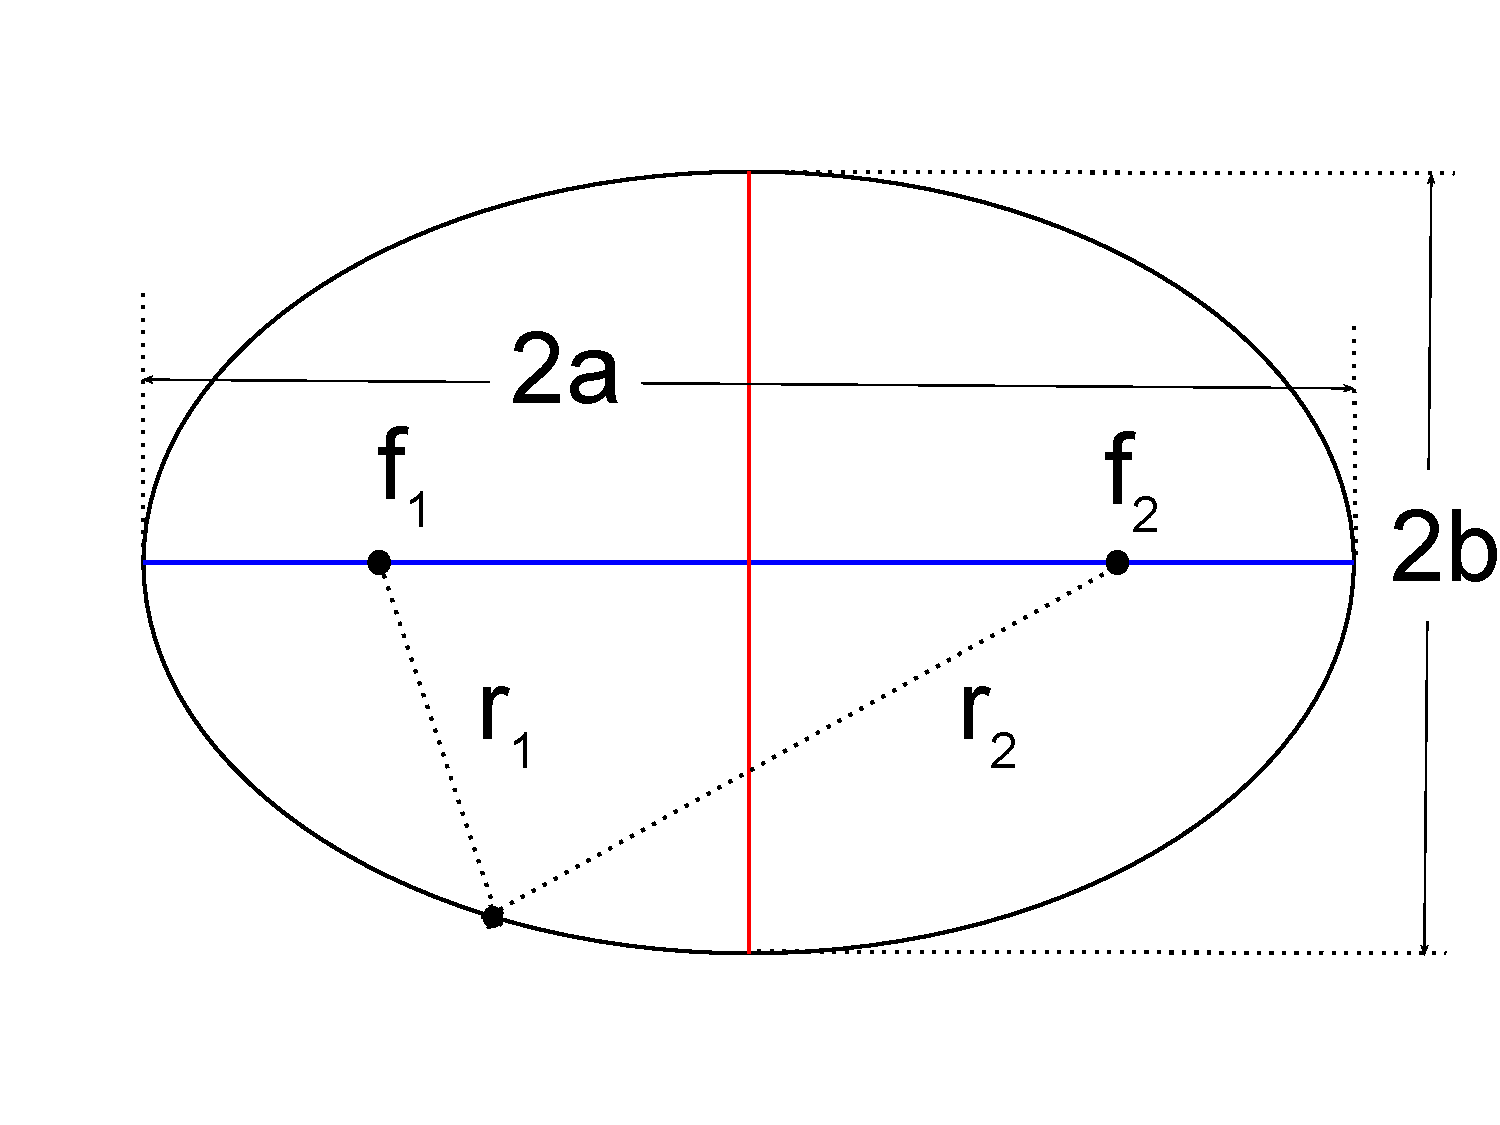
\includegraphics[width=\linewidth]{elipse.pdf}
  \caption{Los planetas recorren una elipse, seg\'un la primera ley de Kepler. El Sol se situar\'\i{}a en uno de los focos. La condici\'on que define la elipse es que la suma de las distancias de cualquiera de sus puntos a sus focos es una cantidad constante: $r_1+r_2 = 2a$.}
  \label{fig:elipse}
\end{marginfigure}

 

\newthought{En primer lugar} descubri\'o que cada planeta se desplaza alrededor del sol siguiento una curva llamada elipse (Figura \ref{fig:elipse}). Una elipse es bastante diferente de un c\'\i{}rculo. Es un tipo de curva que se puede obtener con un trozo de cuerda, dos chichetas y un lapicero. Se sujeta cada uno de los extremos de la cuerda en uno de los focos y la punta del l\'apiz que tensa la cuerda describe una elipse. Desde un punto de vista m\'as preciso la elipse se caracteriza porque los puntos que la forman distan de los focos $f_1$ y $f_2$ una cantidad que sumada es constante ($2a$).  El Sol ya no ocupa la posici\'on central sino que se halla desplazado en uno de los focos.


\newthought{La segunda observaci\'on de Kepler} es tambi\'en experimental y tiene que ver con la velocidad a la que se desplazan los planetas a lo largo de su trayectoria. Kepler propuso que los planetas se mueven m\'as lento cuando se hallan alejados del sol (afelio) y m\'as r\'apido cuando est\'an cerca (perihelio). Pero la segunda ley m\'as all\'a. Lo que dice exactamente es que la l\'\i{}nea imaginaria que unir\'\i{}a cada planeta con el sol recorrer\'\i{}a \'areas iguales en tiempos iguales (Fig. \ref{fig:Kepler_2}). 

\begin{marginfigure}
  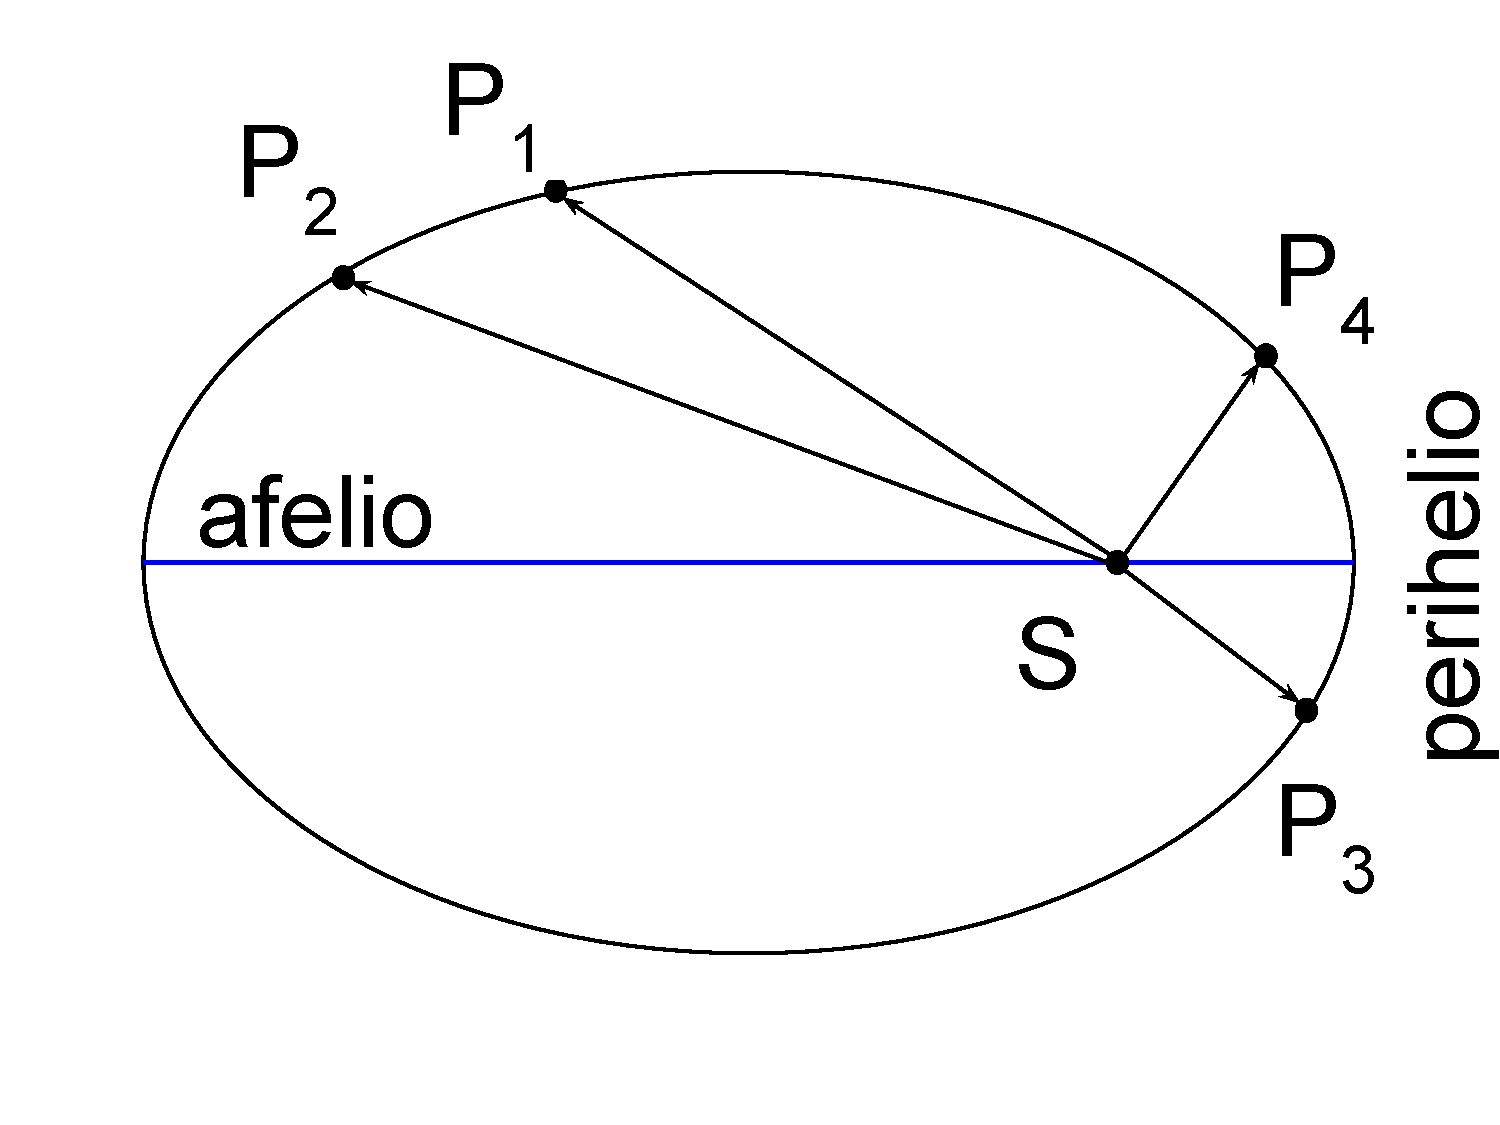
\includegraphics[width=\linewidth]{Kepler_2.pdf}
  \caption{Representaci\'on moderna de la segunda Ley de Kepler. El radio vector que une Sol (S) con el planeta (P) recorre \'areas iguales en tiempos iguales ($SP_1P_2=SP_3P_4$). Como consecuencia la velocidad del planeta es mayor en el perihelio que en el afelio.}
  \label{fig:Kepler_2}
\end{marginfigure}

\newthought{La tercera ley} fue descubierta mucho m\'as tarde que las anteriores y es de una naturaleza distinta ya que compara lo que ocurre con dos planetas. De acuerdo con la misma, cuando se comparan los periodos orbitales y los tama\~{n}os de las \'orbitas de dos de los planetas, los periodos son propocionales a la potencia 3/2 del tama\~{n}o de sus \'orbitas, es decir, si las \'orbita fueran c\'\i{}rculos (en la mayor\'\i{}a de los casos pr\'acticamente lo son), el tiempo necesario para recorrerlo ser\'\i{}a proporcional a la potencia 3/2 del di\'ametro. Como ilustraci\'on pueden observarse los datos recopilados para los diferentes planetas en la Tabla \ref{tab:tercera_ley_kepler}.


\bigskip
\begin{table}[h]
\begin{center}
\footnotesize
\begin{tabular}{lcccc}
\toprule
planeta 	& periodo 		& distancia media & $ T^{2}/R^{3}$ & excentricidad \\
			&   (a\~{n}os)  &  (ua)           & (a\~{n}os$^{2}/ua^{3})$& \\
\midrule
Mercurio 	& 0.241 		& 0.39	 		  & 0.98 	&0.206\\
Venus 		& 0.615 		& 0.72			  & 1.01	&0.007\\
la Tierra   & 1.00   		& 1.00			  & 1.00	&0.017\\
Marte     	& 1.88  		& 1.52			  & 1.01	&0.093\\
J\'upiter   & 11.8   		& 5.20			  & 0.99	&0.048\\
Saturno    	& 29.5  		& 9.54			  & 1.00	&0.054\\
Urano   	& 84.0   		& 19.18			  & 1.00	&0.047\\
Neptuno  	& 165   		& 30.06			  & 1.00	&0.009\\
Plut\'on   	& 248   		& 39.44			  & 1.00	&0.249\\
\addlinespace
\bottomrule
\end{tabular}
\end{center}
\caption{Periodos orbitales, distancia media al Sol y excentricidades para los planetas del Sistema Solar. La distancia media se expresa en unidades astron\'omicas, tomando como 1 la distancia media de la Tierra al Sol ($1.4957  \times 10^{11}$) m. El periodo orbital viene expresado en a\~{n}os terrestres, entendiendo por 1 a\~{n}o terrestre el tiempo que emplea la Tierra en completar una \'orbita alrededor del Sol, ($3.156 \times 10^7$ segundos).}
  \label{tab:tercera_ley_kepler}
\end{table}

Las leyes de Kepler describen c\'omo se
mueven los planetas en sus \'orbitas alrededor del Sol, pero no profundizan acerca de las causas que
provocan ese movimiento. 

\section{La aportaci\'on de Galileo} 
En aquella misma \'epoca Galileo Galilei comenz\'o a estudiar los cielos con su telescopio de refracci\'on. Partiendo de un dise\~{n}o previo del holand\'es Hans Lippershey, Galileo construye en el a\~{n}o 1609 un telescopio de 3x aumentos que perfeccionar\'\i{}a a lo largo de los a\~{n}os siguientes hasta alcanzar los 30x. Gracias a este instrumento realiza importantes descubrimientos tales como que la Luna no posee una superficie lisa sino cubierta de prominencias y oquedades o que las estrellas no se situan en la superficie de una esfera sino a diferentes distancias (el universo parec\'\i{}a por lo tanto tener una inmensa profundidad). Sin embargo, la observaci\'on m\'as relevante de todas fue que J\'upiter pose\'\i{}a cuatro lunas que no giraban entorno a la Tierra. 

Pero el enigma del movimiento segu\'\i{}a sin ser resuelto. ?`Cu\'al es la causa de que los planetas giren? Durante muchos siglos hab\'\i{}a prevalecido el criterio de Arist\'oteles, seg\'un el cual ``el cuerpo en movimiento se detiene cuando la fuerza que lo empuja deja de actuar''. Galileo realiz\'o numerosas observaciones sobre la caida y el movimiento de los cuerpos que le permiteron adquirir una gran intuici\'on acerca de este fen\'omeno. Para entender mejor la soluci\'on encontrada por Galileo, vamos a plantearnos un experimento pensado. Imaginemos un trineo que se desliza por la superficie de un lago helado. Supongamos que en un momento dado dejamos de empujarlo. Sabemos que el trineo recorrer\'a un cierto trayecto antes de pararse. ?`Ser\'\i{}a posible aumentar el trayecto recorrido? La experiencia nos dice que si el hielo fuera muy liso o las cuchillas muy finas el trineo ir\'\i{}a m\'as lejos. Actuando de este modo disminuimos los efectos de lo que se conoce como rozamiento o fricci\'on. Si suponemos que fuera posible disminuir el rozamieno hasta hacerlo desaparecer, en tal caso no habr\'\i{}a nada que se opusiera al movimiento del trineo y \'este se deslizar\'\i{}a hasta el final del lago. Este es el tipo de razonamiento que llev\'o a cabo Galileo, basado en su experiencia, aunque irrealizable desde el punto de vista pr\'actico, dio la clave sobre la que se fundamentar\'\i{}a la mec\'anica del movimiento: si algo se mueve sin que nada lo toque y sin perturbaci\'on alguna, continuar\'a movi\'endose eternamente, siguiendo con velocidad uniforme una l\'\i{}nea recta. Por lo tanto, la velocidad de un cuerpo no es indicio de que sobre \'el act\'uen elementos exteriores.
En palabras del propio Galileo:

\begin{quote}...Toda velocidad, una vez impartida a un cuerpo, se conservar\'a sin alteraci\'on mientras no existan causas externas de aceleraci\'on o frenado, condici\'on que se cumple solamente sobre los planos horizontales; pues el movimiento de un cuerpo que cae por una pendiente se acelera, mientras que el movimiento hacia arriba se frena; de esto se infiere que el movimiento sobre un plano horizontal es perp\'etuo; pues, si la velocidad es uniforme, no puede disminuirse o mermarse, y menos a\'un destruirse.\cite{GalileoTwoNewSciences}
\end{quote}

La gran aportaci\'on de Galileo es intuir que la clave en la explicaci\'on del fen\'omeno del movimiento consiste en relacionar la acci\'on de elementos externos con el cambio de la velocidad (y no con la velocidad misma).

\section{La s\'\i{}ntesis de Newton}

La conclusi\'on de Galileo, que es la correcta, la reformul\'o a\~{n}os m\'as tarde Isacc Newton con el nombre de Principio de Inercia.  Si un cuerpo aumenta su velocidad significa que una fuerza ha sido aplicada en la direcci\'on del movimiento. Del mismo modo una fuerza aplicada en una direcci\'on distinta puede cambiar la direcci\'on en la que un cuerpo se mueve. La base de la mec\'anica cl\'asica vendr\'a dada por la relaci\'on entre fuerza y  aceleraci\'on y no entre fuerza y velocidad. Newton introduce el concepto de ``fuerza'', una representaci\'on matem\'atica desprovista de cualquier otra connotaci\'on, simple y manejable.

 Pero, ?`qu\'e es exactamente una fuerza? El concepto surge de nuestra sensaci\'on de esfuerzo cuando empujamos o estiramos de un objeto. Pero su generalizaci\'on va mucho m\'as all\'a del esfuerzo humano. Newton era  especialmente bueno generalizando tal y como demuestra en sus Principia\cite{Newton1687}:
\begin{quote}Una fuerza exterior es una acci\'on que se ejerce sobre un cuerpo, con el objeto de modificar su estado, ya de reposo, ya de movimiento rectil\'\i{}neo y uniforme. La fuerza consiste \'unicamente en su acci\'on y no permanece en el cuerpo cuando deja de actuar aqu\'ella. Pues un cuerpo se mantiene en cualquier nuevo estado que adquiera, gracias a su ``vis inertiae'' \'unicamente. Las fuerzas pueden ser de origen muy distinto, tales como la percusi\'on, presi\'on o fuerza centr\'\i{}fuga.
\end{quote}

Esta generalizaci\'on permitir\'a extender el alcance de la mec\'anica hasta crear un marco universal, un sistema coherente que abarca desde el movimiento de los cuerpos en la Tierra  hasta el de los planetas. Para resolver este puzle Newton contaba con dos piezas claves: las tres leyes de Kepler sobre el movimiento planetario y los descubrimientos de Galileo sobre c\'omo los cuerpos se mueven en la Tierra. Pese a su aparente afinidad tem\'atica, estos componentes no parec\'\i{}an ser compatibles. Para la mayor\'\i{}a de los cient\'\i{}ficos de la \'epoca el origen del movimiento de los planetas en sus \'orbitas no ten\'\i{}a nada que ver con la causa de los movimientos de los cuerpos terrestres. La distinci\'on entre el mundo terrenal y la esfera celeste segu\'\i{}a funcionado en las mentes.

Newton funda la din\'amica sobre sus tres leyes del movimiento:

\newthought{La primera ley de Newton} que es, como ya se ha comentado, la reformulaci\'on del principio enunciado por Galileo dice as\'\i{}:``Todo cuerpo contin\'ua en un estado de reposo o de movimiento uniforme en l\'\i{}nea recta a menos que sea obligado a cambiar ese estado por fuerzas impuestas sobre \'el.'' As\'\i{}, si sobre un cuerpo no act\'ua ninguna fuerza, seguir\'a movi\'endose uniformemente tanto en velocidad como en direcci\'on.

\newthought{La segunda ley} afirma que: ``...el cambio de movimiento [de un cuerpo] es proporcional a la fuerza imprimida y se efect\'ua en la direcci\'on de la l\'\i{}nea recta en que es imprimida esa fuerza.'' Newton adapta la idea de Galileo de que la aceleraci\'on del movimiento de un cuerpo es la magnitud clave. Pero va m\'as all\'a e introduce el concepto de fuerza ``centr\'\i{}peta'', una fuerza dirigida hacia el centro, para distinguirla del concepto introducido por el otro gran cient\'\i{}fico de la \'epoca, Christiaan Huygens, de fuerza centr\'\i{}fuga. Cuando hacemos girar una piedra atada con una cuerda, la mano que la sujeta debe tirar de la cuerda para contrarrestar la tensi\'on y mantener la piedra en su \'orbita. Igualmente importante es la introducci\'on del concepto de ``masa'', la cantidad de materia en un cuerpo, distinta aunque proporcional a su peso. La masa se puede medir, permanece constante, independientemente de la posici\'on o del movimiento (al menos hasta que en pleno siglo XX Einstein introduzca su teor\'\i{}a de la relatividad).

\newthought{La tercera ley}, a diferencia de las dos anteriores, es completamente debida a Newton. Afirma que: ``...a cada acci\'on hay siempre opuesta otra reacci\'on igual: o, la acci\'on m\'utua de dos cuerpos el uno sobre el otro es siempre igual y dirigida a las partes contrarias.'' 

% * <alopezpo@gmail.com> 2015-01-17T19:06:21.040Z:
%
%  Gráfica piedra girando en %circulo
%
Podemos entender las tres leyes mediante un ejemplo gr\'afico\cite{Kepler-second-law-gif}. Supongamos que somos los afortunados en un sorteo y nos ha tocado un viaje a la estaci\'on espacial. Imaginemos que hacemos girar una piedra atada a una cuerda. Esta piedra describe una circunferencia ya que con nuestra mano compensamos la fuerza centr\'\i{}fuga (tercera ley). La piedra gira en una trayectoria circular, por lo que sobre la piedra tendr\'\i{}a que actuar constantemente una fuerza central que la mantenga girando en un c\'\i{}rculo. La piedra curva constantemente su trayectoria porque la cuerda le impide salir por la tangente (literalmente hablando) (segunda ley). Si en un momento dado la cuerda se rompiese, la piedra saldr\'\i{}a disparada tangencialmente . De acuerdo con el principio de inercia (primera ley) la piedra seguir\'\i{}a eternamente una trayectoria rectil\'\i{}nea, o al menos el tiempo suficiente  hasta alcanzar en la ceja al cosmonauta ruso (dejemos para m\'as tarde la resoluci\'on del incidente diplom\'atico).

 \begin{marginfigure}
  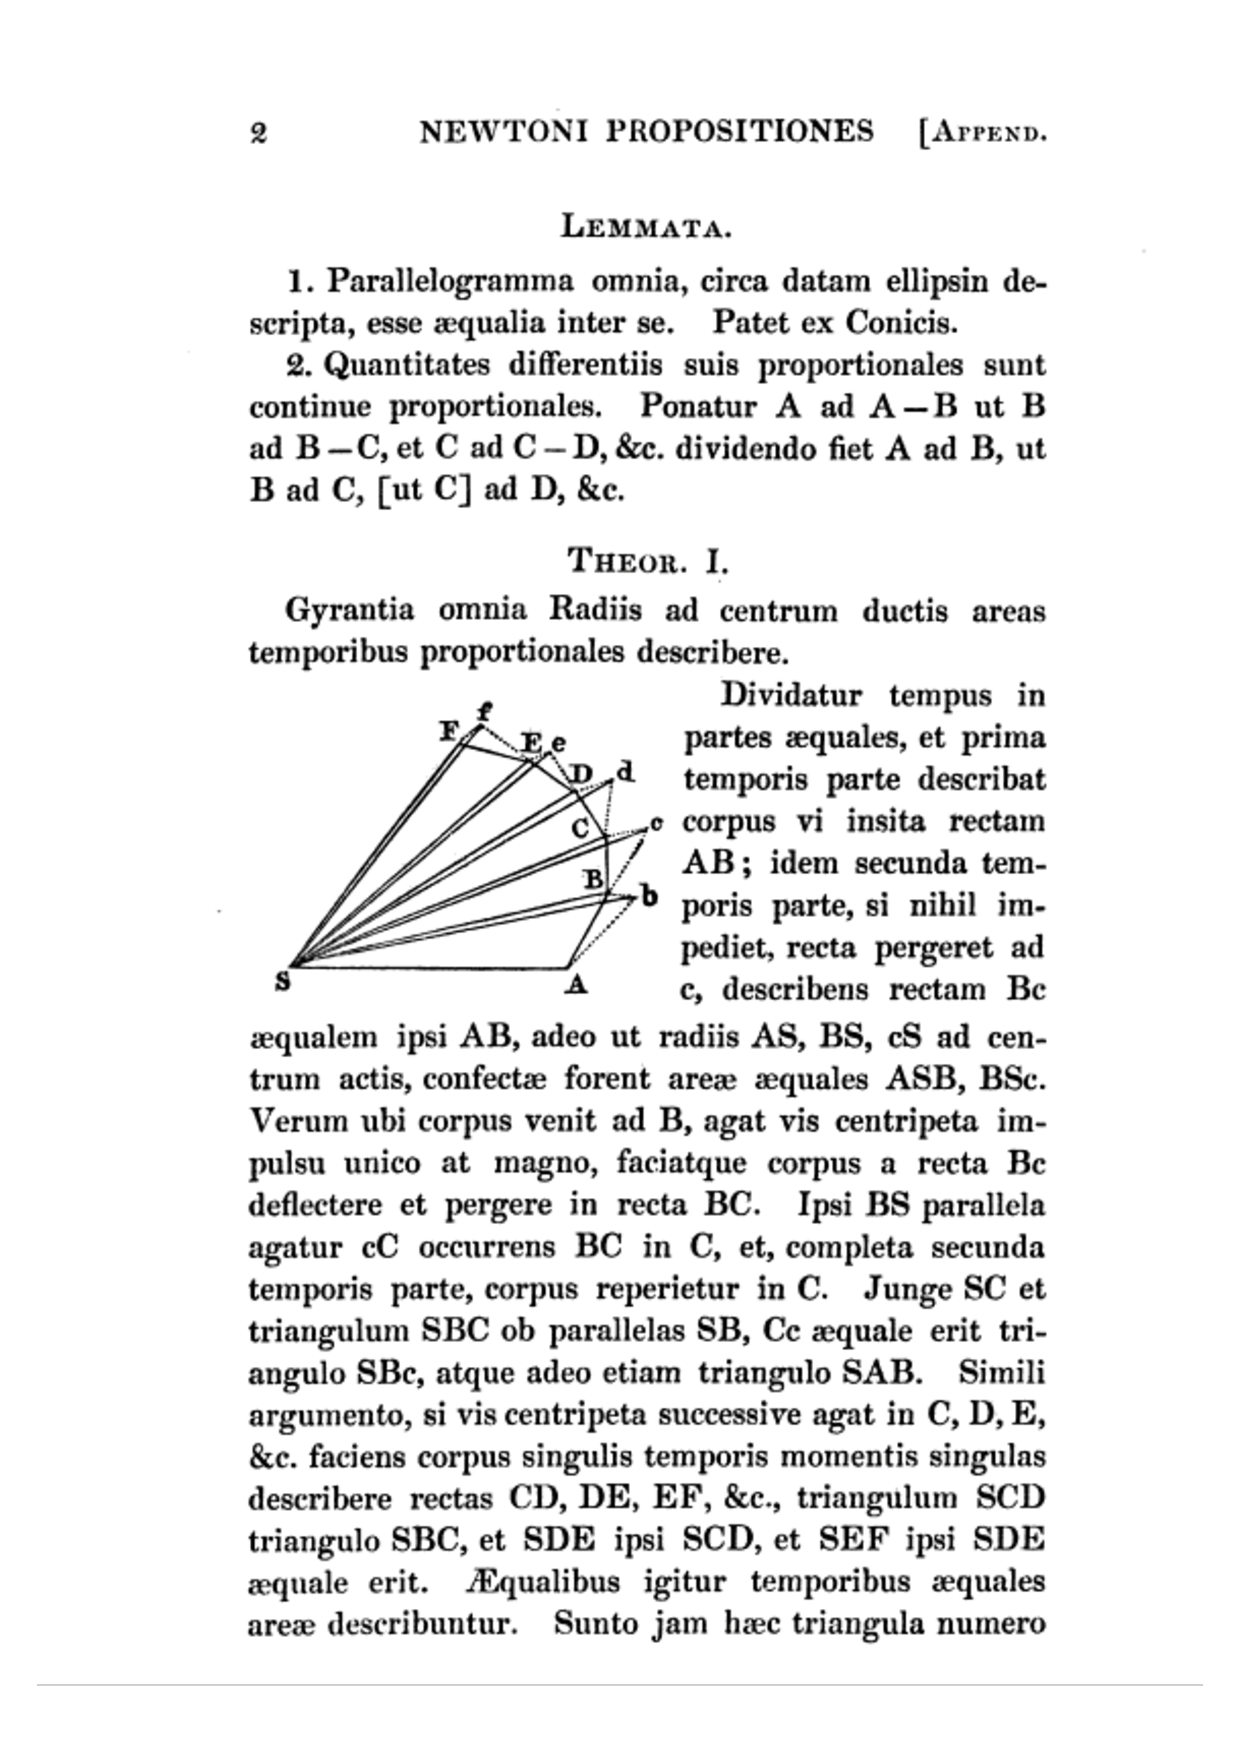
\includegraphics[width=\linewidth]{figuraNewton.pdf}
  \caption{P\'agina de ``De Motu corporum in gyrum'' en la que Newton utiliza una aproximaci\'on discreta, reemplazando el efecto de una fuerza cont\'\i{}nua por una sucesi\'on de impulsos que se suceden a int\'ervalos regulares de tiempo.
\url{http://www.newtonproject.sussex.ac.uk/view/texts/normalized/NATP00089}}
  \label{fig:Newton_1}
\end{marginfigure}



 Newton estim\'o que los planetas no precisan de una fuerza que les impulse a lo largo de su trayectoria sino de una atracci\'on de car\'acter central cuyo origen radicar\'\i{}a en el Sol. Prob\'o que el hecho mismo de que los planetas cubran \'areas iguales en tiempos iguales implica necesariamente que la fuerza tiene que ir dirigida hacia el Sol. La demostraci\'on moderna de este hecho suele realizarse mediante el c\'alculo diferencial que el propio Newton y Leibniz desarrollaron, haciendo uso de una formulaci\'on  que involucra las leyes de conservaci\'on\cite{tagkey1976iv}. Sin embargo, cuando Newton discute este punto en su obra ``De Motu corporum in gyrum'' (1684) no utiliza ese tipo de herramientas matem\'aticas sino que recurre al diagrama de la  Figura \ref{fig:Newton_1}. 
 

Utilizaremos una versi\'on actualizada del diagrama (Fig. \ref{fig:keplerFromNewton}) para entender el razonamiento. Supongamos un planeta que en su trayectoria recorre los puntos A, B y C. La fuerza central act\'ua sobre \'el de forma puntual y hace que cambie de direcci\'on, de tal forma que ya no seguir\'a su trayectoria prevista Bc sino BC. Es decir, la actuaci\'on discreta de la fuerza central va cambiando la trayectoria.


%%%%%%%%%%%%%%%
\begin{figure*}[h]
  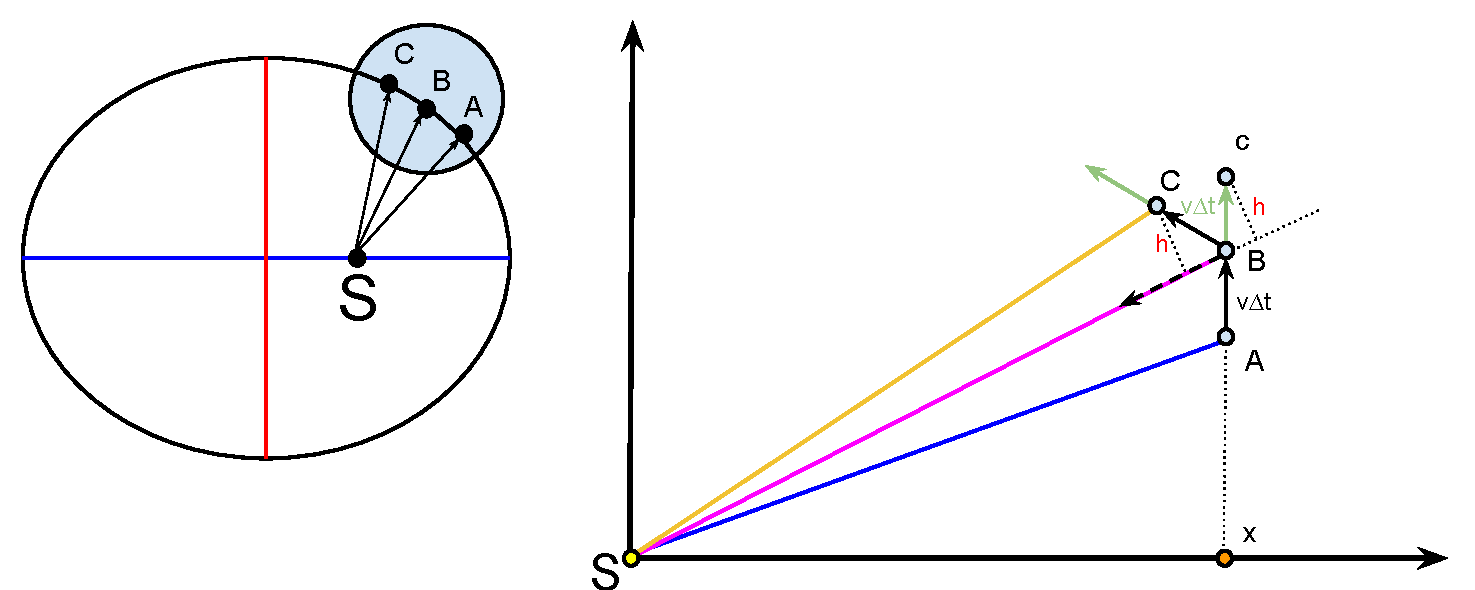
\includegraphics[width=\linewidth]{leyKeplerfromNewton.pdf}%
  \caption{El Sol ejerce una fuerza central puntual que desv\'\i{}a el cuerpo de su trayectoria original, de tal forma que ya no llega hasta el punto c sino al punto C.}
  \label{fig:keplerFromNewton}%
\end{figure*}
%%%%%%%%%%%%%%%



Observando con detalle la figura \ref{fig:keplerFromNewton}, se ve que las \'areas de los tri\'angulos $ABS$ y $BcS$ son iguales ya que poseen la misma base ($v\Delta t$) y la misma altura (Sx):

\begin{equation}
ABS=\frac{1}{2}(v\Delta t) \overline{Sx}=BcS
\label{eq:areaIgual_1}
\end{equation}

Por otra parte el \'area del nuevo tri\'angulo $BCS$ es la misma que la del tri\'angulo $BcS$ que se hubiera formado si la fuerza no hubiera actuado. En efecto:

\begin{equation}
BCS =\frac{1}{2}h\overline{SB}=BcS
\label{eq:areaIgual_2}
\end{equation}


De las ecuaciones \ref{eq:areaIgual_1} y \ref{eq:areaIgual_2} se sigue que la aplicaci\'on de una fuerza central  desv\'\i{}a el cuerpo de su trayectoria original, pero el area de cada tri\'angulo $BCS$ es siempre id\'entica a la del tri\'angulo original $ABS$, es decir, la segunda ley de Kepler.

Si el \'angulo $\theta$ recorrido por r se hace suficientemente peque\~{n}o, tal y como se muestra en la fig. \ref{fig:fuerzaCentripeta}, por tri\'angulos semejantes se puede ver que
\begin{equation}
\frac{\overline{BC}}{r}=\frac{\Delta v}{v}
\label{eq:incremento_v}
\end{equation}

%%%%%%%%%%%%%%%
\begin{figure*}[h]
  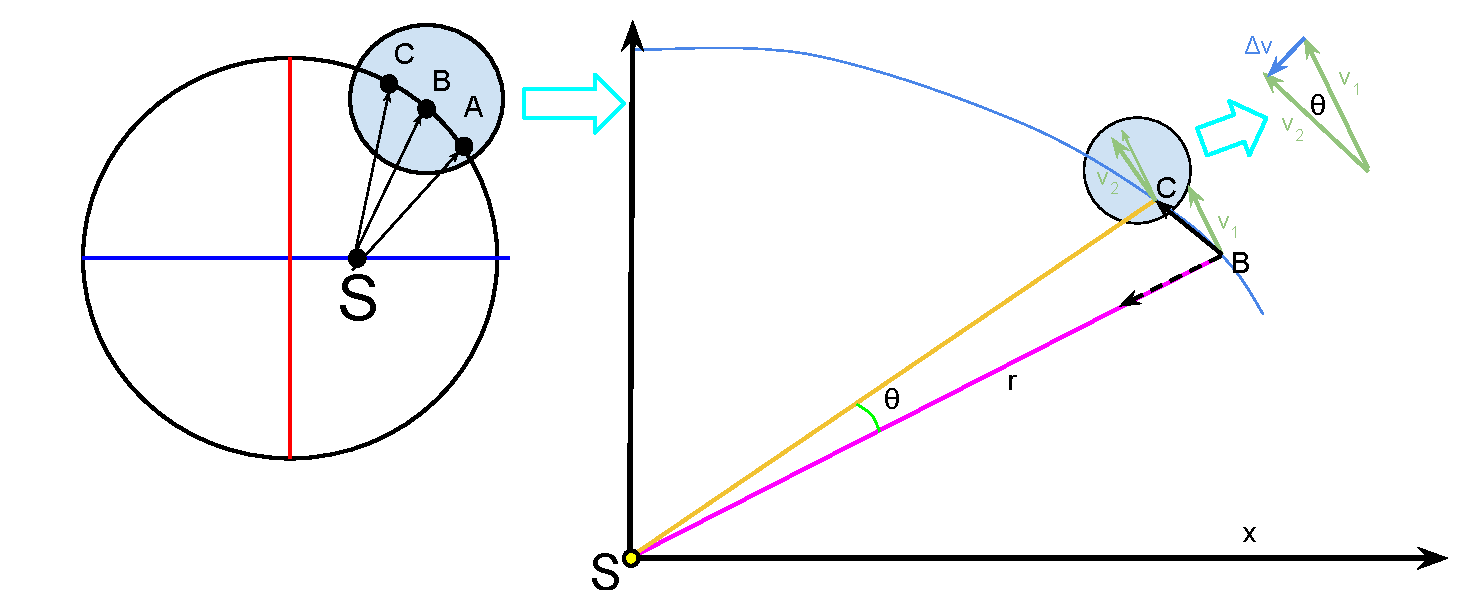
\includegraphics[width=\linewidth]{FuerzaCentripeta.pdf}
  \caption{Si el \'angulo $\theta$ es suficientemente peque\~{n}o, los tri\'angulos $SBC$ y $v_{1}v_{2}\Delta v$ son semejantes.}
  \label{fig:fuerzaCentripeta}
\end{figure*}
%%%%%%%%%%%%%%%
El espacio recorrido es, por definici\'on, el producto de la velocidad por el tiempo empleado, $\overline{BC}=v\Delta t$. Si sustituimos esta expresi\'on en la ecuaci\'on \ref{eq:incremento_v} y despejamos $\Delta v$ obtenemos

\begin{equation}
\Delta v=\frac{v^{2}\Delta t}{r}
\label{eq:incremento_v_2}
\end{equation}

Si definimos la aceleraci\'on como el incremento de la velocidad  en un cierto tiempo $\Delta t$ y utilizamos la ec. \ref{eq:incremento_v_2}
\begin{equation}
a_{n}=\frac{\Delta v}{\Delta t}=\frac{v^{2}}{r}
\label{eq:aceleracion_n2}
\end{equation}
La fuerza central que actuar\'a sobre el cuerpo, suponiendo que tenga una masa $m$ ser\'a
\begin{equation}
F_{n}=m\frac{v^{2}}{r}
\label{eq:fuerza_centripeta}
\end{equation}
y se denomina \emph{fuerza normal} o \emph{centr\'\i{}peta}.


Es posible demostrar de forma intuitiva que las leyes de Kepler se derivan de las leyes de Newton en una geometr\'\i{}a eucl\'\i{}dea\cite{Goodstein1996}\cite{Beckman2006}\cite{ANU:7701776}.


\section{Ley de la gravitaci\'on de Newton}
Newton sab\'\i{}a que el origen del movimiento planetario se debe a la existencia de una fuerza central dirigida hacia el Sol. A medida que aumenta la distancia entre el planeta y el Sol disminuye la fuerza que los atrae. Si comparamos dos planetas situados a diferentes distancias del Sol es posible demostrar que la atracci\'on gravitatoria debe de ser inversamente proporcional al cuadrado de la distancia.  La demostraci\'on de este hecho se simplifica mucho para el caso particular de una trayectoria circular. Un c\'\i{}rculo, al fin y al cabo, puede ser considerado un caso particular de elipse en el que los dos focos coinciden en el centro. Si definimos el periodo $P$ como el tiempo que emplea el planeta en completar una vuelta, la velocidad ser\'a
\begin{equation}
v=\frac{2\pi r}{P} 
\label{eq:periodo}
\end{equation}
Pero la tercera ley de Kepler en el caso especial de una \'orbita circular dice que $P^{2}=kr^{3}$. Por lo tanto la fuerza centr\'\i{}peta (ec. \ref{eq:fuerza_centripeta}) ser\'a igual a
\begin{equation}
F=\frac{4\pi^{2}m}{kr^{2}} \propto \frac{1}{r^{2}}
\label{eq:gravitacion_1}
\end{equation}
Es decir, la fuerza central tienen que ser proporcional al inverso del cuadrado de la distancia tal y como Newton confirm\'o a Halley en su visita.

\begin{marginfigure}
  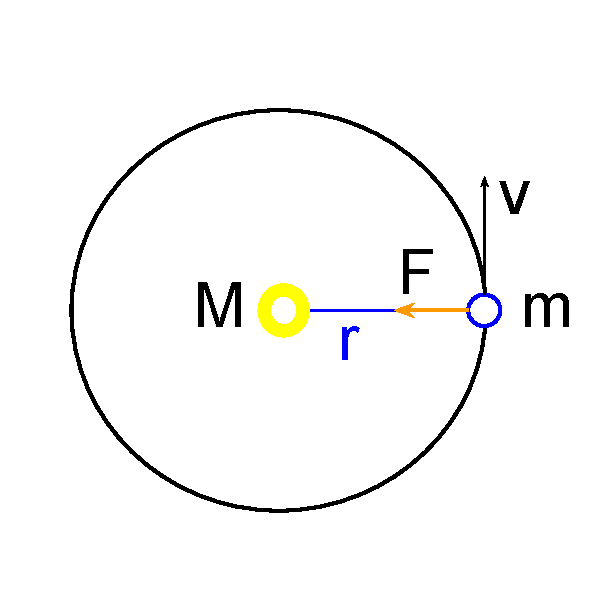
\includegraphics[width=\linewidth]{FuerzaCentripetaCirculo.pdf}
  \caption{Movimiento de un cuerpo de masa $m$ bajo la interacci\'on gravitatoria con $M$.}
  \label{fig:MovimientoCircular}
\end{marginfigure}

 

\begin{quote}
Todo objeto en el universo atrae a cualquier otro con una fuerza proporcional a la masa de cada uno e inversamente proporcional al cuadrado de la distancia que los separa
\end{quote}
\begin{equation}
F=G\frac{mM}{r^{2}} 
\label{eq:gravitacion_2}
\end{equation}
La demostraci\'on es m\'as compleja para el caso general de \'orbitas el\'\i{}pticas. 

El talento de Newton consisti\'o en establecer que la interacci\'on gravitatoria era una propiedad universal: cualquier cuerpo en el espacio o en la Tierra experimenta una atracci\'on de estas caracte\'\i{}sticas.

\section{Masa inercial y masa gravitacional}
El concepto de masa ha aparecido de dos formas diferentes. Por una parte hemos visto que la masa es la constante que relaciona la fuerza que aplicamos sobre un cuerpo con la aceleraci\'on que experimenta. Si sobre dos masas en reposo act\'uan dos fuerzas id\'enticas durante un cierto tiempo y al finalizar la velocidad de una resulta ser el triple que la de la otra, concluimos que la primera tiene una masa (inercial) tres veces menor que la segunda. En este experimento la gravedad no juega ning\'un papel ya que es la misma a lo largo de todo el movimiento. 

El otro contexto en el que aparece la idea de masa es en el de la atracci\'on gravitatoria. Mediante una balanza podemos hallar la masa (gravitatoria) de un cuerpo compar\'andola con la masa conocida de otros que experimentan la misma atracci\'on (las pesas). Tenemos dos modos distintos de obtener la masa. La pregunta que surge de forma inmediata es si los valores obtenidos por uno u otro m\'etodo coinciden. Desde los experimentos de Galileo la experiencia nos dice que s\'\i{}, ambas coinciden. Este hecho, que parece casual y sin mayor trascendencia en la mec\'anica cl\'asica adquir\'o un papel central en la revisi\'on que llev\'o a cabo Einstein en su teor\'\i{}a general de la relatividad. De acuerdo con Newton, el efecto gravitacional es instant\'aneo, esto es, si movemos una masa sentir\'\i{}amos instant\'aneamente una nueva fuerza debida a la nueva posici\'on de la masa. Si esto fuera as\'\i{} la informaci\'on sobre la posici\'on de la masa podr\'\i{}a viajar a una velocidad superior a la de la luz. Einstein anticip\'o argumentos que sugieren que la velocidad de la luz es insuperable, por lo que se hac\'\i{}a necesario modificar la ley de la gravitaci\'on. En palabras de Einstein:

\begin{quote}
Al cabo de tres siglos tuvimos que volver al problema inicial del movimiento y revisar el procedimiento de investigaci\'on, descubrir detalles que pasaron inadvertidos, adquirendo as\'\i{} una nueva imagen del Universo que nos rodea\cite{Einstein1938}.
\end{quote}






\section{Campo gravitatorio}
La influencia de Newton en sus contempor\'aneos fue enorme. Su explicaci\'on de los movimientos debidos a la gravedad caus\'o una honda impresi\'on en las generaciones posteriores de cient\'\i{}ficos. La din\'amica basada en la idea de fuerza a distancia era capaz de explicar con precisi\'on el movimiento de los cuerpos que interact\'uan cuando no est\'an muy alejados y tienen caracter puntual.
Sin embargo, si las distancias aumentan, la idea de propagaci\'on instant\'anea resultaba dif\'icil de aceptar, incluso para el propio Newton. A lo largo de su vida Newton bascular\'a desde ideas puramente mecanicistas en las que parece encajar este hecho (que los cuerpos puedan interactuar sin ning\'un intermediario a pesar de la distancia) hasta otras en las que muestra su incapacidad para explicar la verdadera naturaleza de la gravedad. En su carta al reverendo Bentley en 1693, Newton reconoce\cite{NewtonBentleyLetter1693}:
\begin{quote}
Usted habla a veces de la gravedad como esencial e inherente a la materia. Por favor, no me adscriba a m\'\i{} esa idea; porque la causa de la gravedad no pretendo conocerla, y por consiguiente habr\'\i{}a de tomarme más tiempo para dar cuenta de ella.
\end{quote}

Imaginemos que situamos una masa testigo (un astronauta, por ejemplo) a una cierta distancia de la Tierra. A medida que el astronauta se aleja de la superficie terrestre, la fuerza con la que se sentir\'a atraido por el planeta disminuir\'a, tal y como se muestra en la tabla \ref{tab:gravedad_altura}. 

\bigskip
\begin{table}[h]
\begin{center}
\footnotesize
\begin{tabular}{ccc}
\toprule
altura	& aceleraci\'on de la gravedad & peso de una persona \\
(km)    &   ($m/s^2$)   			   &  (100 Kg)           \\
\midrule
0	& 9.75 		& 100	\\
6437& 2.44 		& 25	\\
12874& 1.09   	& 11	\\
19312& 0.61  	& 6.2	\\
25749& 0.39   	& 4	\\
32186& 0.27  	& 2.8	\\
38623& 0.18   	& 2	\\
\addlinespace
\bottomrule
\end{tabular}
\end{center}
\caption{Variaci\'on de la fuerza de la gravedad con la distancia a la superficie terrestre. La primera columna indica la distancia a la superficie terrestre. La segunda muestra la aceleraci\'on de la gravedad a esas distancias. Por \'ultimo se muestra c\'omo variar\'\i{}a el peso de una persona (100 Kg) al alejarse de la Tierra.}
  \label{tab:gravedad_altura}
\end{table}

La presencia de una masa (el planeta Tierra, por ejemplo) en el espacio crea una propiedad en torno a ella que se pone de manifiesto cuando colocamos otra masa de testigo (nuestro solitario astronauta). Esta segunda masa, llamada \emph{masa de prueba} ser\'a atraida por la masa original seg\'un la recta que une los centros de ambos cuerpos. En la fig. \ref{fig:campo_gravitatorio} las l\'\i{}neas representan las direcciones de las fuerzas que experimentar\'\i{}a la masa de prueba situada en diferentes puntos
\begin{marginfigure}
  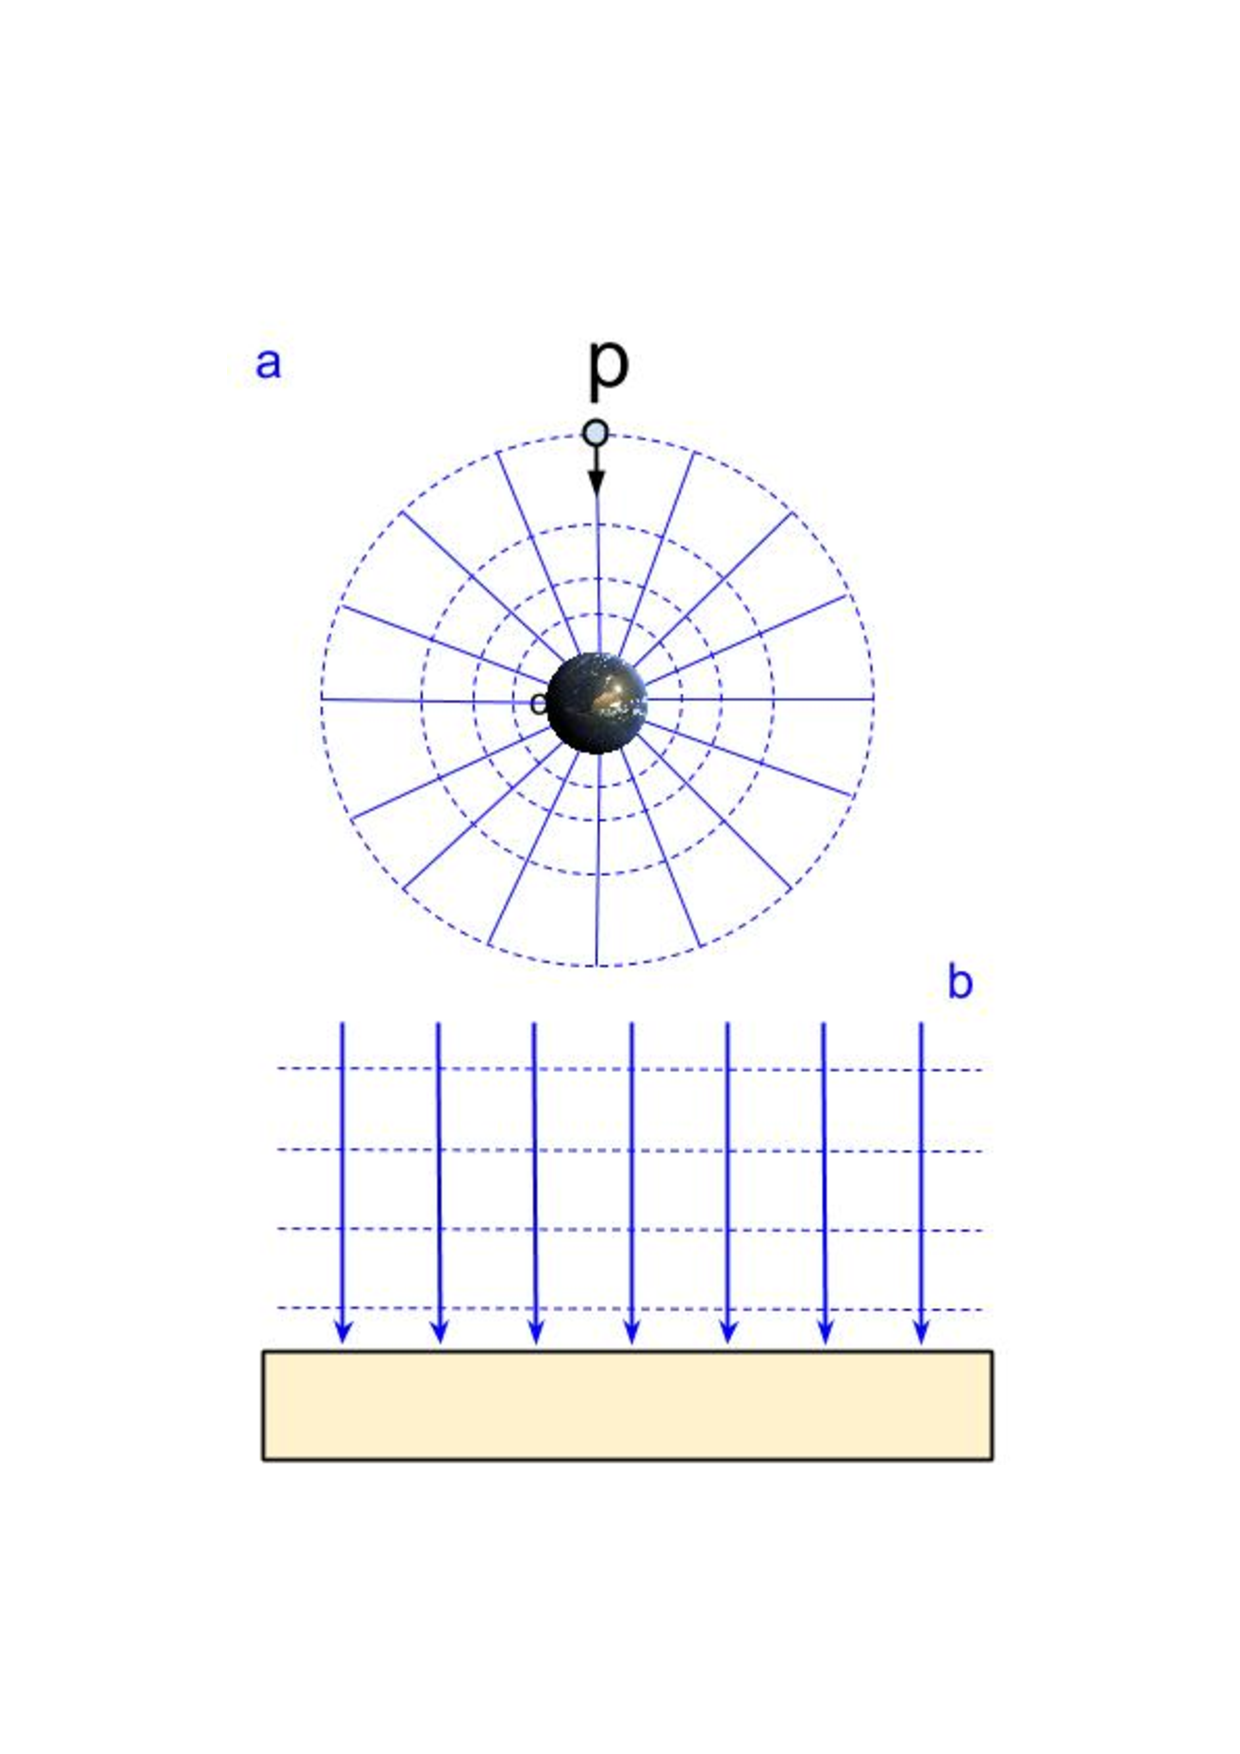
\includegraphics[width=\linewidth]{campo_gravitatorio.pdf}
  \caption{Representaci\'on del campo gravitatorio terrestre. Las l\'\i{}neas cont\'\i{}nuas representan las l\'\i{}ineas de campo. Los c\'\i{}rculos discont\'\i{}nuos son las superficies equipotenciales. En puntos suficientemente alejados de la Tierra (a) las l\'\i{}neas de campo se van separando a medida que la intensidad del campo decrece. En la superficie de la Tierra (b) la intesidad del campo es pr\'acticamente constante.}
  \label{fig:campo_gravitatorio}
\end{marginfigure}
Estas l\'\i{}neas se denominan \emph{l\'\i{}neas de fuerza del campo gravitatorio}. El conjunto total de las l\'\i{}neas de fuerza, o, m\'as brevemente, el campo, indica c\'omo se comportar\'\i{}a un cuerpo de prueba colocado en las proximidades. Las l\'\i{}neas de fuerza son perpendiculares a la superficie de la Tierra y de cualquier esfera conc\'entrica. Por lo tanto su densidad es mayor en la proximidad de la superficie y disminuye a medida que se alejan. Resumiendo, las l\'\i{}neas de fuerza cumplen una funci\'on doble. Por una parte indican la direcci\'on de la fuerza que experimentar\'\i{}a un cuerpo colocado en sus inmediaciones. Por otra parte su densidad en el espacio representa la variaci\'on de la fuerza con la distancia. 

Habr\'a que esperar hasta el siglo XIX para que la noci\'on de campo haga su primera aparici\'on como un t\'ermino t\'ecnico en la mente de Michael Faraday y en el contexto de los campos el\'ectricos, como veremos en el cap\'\i{}tulo \ref{ch:electromagnetismo}


Si en la ec. \ref{eq:gravitacion_2} separamos la masa testigo del resto de las variables, a las que englobamos en la aceleraci\'on $g$, se obtiene la expresi\'on para el peso del cuerpo

\begin{equation}
P \equiv F=mg 
\label{eq:definicion_peso}
\end{equation}

Obviamente el peso cambia con la distancia pero la masa es inherente al cuerpo y permanece siempre la misma.


El concepto de campo gravitatorio aparentemente no supone ninguna ventaja con respecto al plantemiento original de Newton de fuerzas que act\'uan sobre cuerpos puntuales. 



\section{Campos de fuerza conservativos}
La b\'usqueda de la permanecia y la inmutabilidad subyace en muchas de las controversias que se sucedieron entre los cient\'\i{}ficos de la \'epoca. Para Leibniz, era el producto de la masa por el cuadrado de la velocidad del cuerpo en movimiento lo que permanec\'\i{}a inmutable. Esto le llev\'o a una pol\'emica con Descartes y el propio Newton que afirmaban que la magnitud que se conservaba era el producto de la masa por la velocidad\cite{Cajori1899}. Es muy posible que la disputa se debiera a la falta de claridad en el concepto de masa y su distinci\'on del peso. ?`Qu\'e se conservaba realmente? La segunda Ley de Newton permite deducir la conservaci\'on del momento, que se define como
\begin{equation}
\vec{p}\equiv m\vec{v}\Rightarrow\frac{d\vec{p}(t)}{dt}=m\frac{d\vec{v}(t)}{dt}=m\vec{a}=\vec{F}
\label{eq:definicion_momento}
\end{equation}


Pero si tomamos el punto de vista de Leibniz, lo que se conserva es una magnitud muy distinta, ser\'a lo que mucho m\'as tarde se llamar\'a energ\'\i{}a. 

Supongamos que una fuerza $\vec{F}(t)$ act\'ua sobre una part\'\i{}cula que se desplaza desde $\vec{r_1}=\vec{r}(t_1)$ hasta $\vec{r_2}=\vec{r}(t_2)$. 
\begin{marginfigure}
  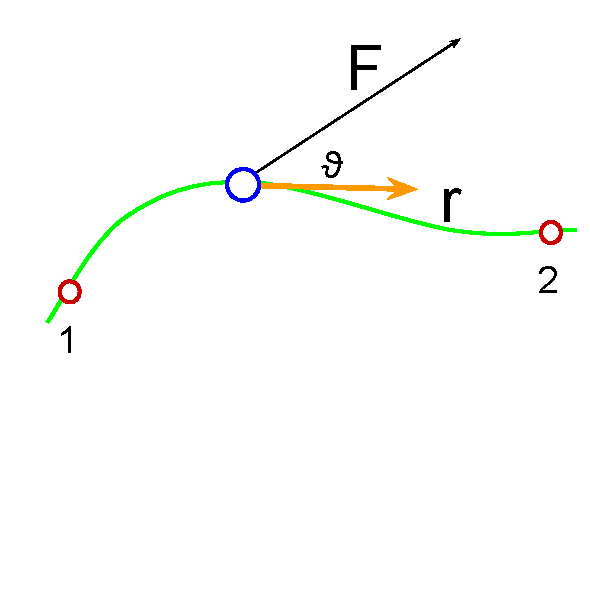
\includegraphics[width=\linewidth]{TrabajoParticulaPuntual.pdf}
  \caption{Trabajo realizado por la fuerza F actuando sobre la part\'\i{}cula que se desplaza a lo largo de una curva de 1 a 2.Obs\'ervese que s\'olo la componente tangencial de la fuerza realiza trabajo sobre la part\'\i{}cula}
  \label{fig:trabajo_particula}
\end{marginfigure}
Definimos el trabajo realizado por la fuerza sobre la part\'\i{}cula como: 

\begin{equation}
W_{12}=\int_{t_1}^{t_2} \vec{F}(t)d\vec{r}
\label{eq:definicion_trabajo}
\end{equation}

La ec. \ref{eq:definicion_trabajo} es una ecuaci\'on de l\'\i{}nea. La idea es integrar la proyecci\'on de la fuerza sobre la direcci\'on instant\'anea del movimiento. Si multiplicamos y dividimos por $dt$ con el fin de hacer m\'as clara la expresi\'on

\begin{equation}
W_{12}=\int_{t_1}^{t_2} \vec{F}(t)\frac{d\vec{r}}{dt}dt=\int_{t_1}^{t_2} \vec{F}(t)\vec{v}(t)dt
\label{eq:definicion_trabajo_2}
\end{equation}

Si utilizamos la ec. \ref{eq:definicion_momento} para sustituir $\vec{F}(t)$ por la derivada del momento y tenemos en cuenta las propiedades del producto escalar\footnote{$d(\vec{a}\cdot \vec{b})=d\vec{a}\cdot \vec{b}+\vec{a}\cdot d\vec{b}$}
\begin{equation}
W_{12}=\int_{t_1}^{t_2} \frac{d\vec{p}}{dt}\frac{\vec{p}}{m}dt=\frac{1}{m}\int_{p_1}^{p_2}d(\vec{p}\cdot \vec{p})-\vec{p}\cdot d \vec{p}
\label{eq:definicion_trabajo_2}
\end{equation}
por lo que finalmente resulta
\begin{equation}
W_{12}=\frac{(p_2)^2}{2m}-\frac{(p_1)^2}{2m}\equiv T_2-T_1
\label{eq:definicion_energia_cinetica}
\end{equation}
donde hemos definido la energ\'\i{}a cin\'etica como $p^2/2m$ o $mv^2/2$. El trabajo efectuado  es igual a la variaci\'on de la energ\'\i{}a cin\'etica. \'Unicamente la componente tangencial de la fuerza  es la que realiza un trabajo. Esa componente acelera la part\'\i{}cula a lo largo de su trayectoria y por lo tanto es capaz de aumentar su energ\'\i{}a cin\'etica, tal y como se puede ver en la figura \ref{fig:trabajo_particula}.

Cuando el campo de fuerzas es tal que el trabajo $W_{12}$ es el mismo independientemente del camino recorrido, diremos que la fuerza es \emph{conservativa}. Otra consecuencia de esta definici\'on es que si desplazamos la part\'\i{}cula a lo largo de una circuito cerrado en un campo de fuerzas conservativo, el trabajo realizado ser\'a nulo
\begin{equation}
\oint \vec{F}(t)d\vec{r}=0
\label{eq:trabajo_cerrado}
\end{equation}


%Energía potencial. Conservación de la energía total


%%Polémica de la "Vis Viva"
%http://www.jstor.org/discover/10.2307/228103?sid=21105524335451&uid=2&uid=4&uid=3737952
%%
%
%Linea del tiempo del concepto de campo Kepler->Newton/Leibniz->Kant->Faraday->Maxwell->Einstein
%
% * <alopezpo@gmail.com> 2015-03-04T08:32:44.667Z:
%
%  El término "campo", hizo su primera aparición en la física como un término técnico en la mitad del siglo XIX. Pero la noción de lo que más tarde llegó a ser llamado un campo había sido un largo tiempo en gestación. Las primeras discusiones del magnetismo y de la causa de las mareas del océano tenían hace mucho tiempo sugirieron la idea de una "zona de influencia" que rodea a ciertos cuerpos. Representación matemática de Johannes Kepler del movimiento orbital de Marte le animó a formular lo que llamó "una verdadera teoría de la gravedad" que implica la noción de la atracción. Isaac Newton llegó a construir una dinámica eminentemente eficaces, con la atracción como su ejemplo principal de la fuerza. La suya era una teoría del campo? Los historiadores de la ciencia no están de acuerdo. Mucho depende de si una teoría coherente con la idea de la acción a distancia debería calificar como una teoría "campo". Roger Boscovich e Immanuel Kant más tarde tomaron el concepto newtoniano de la atracción en nuevas direcciones. Se dejó a Michael Faraday para proponer la "existencia física" de las líneas de fuerza y ​​de James Clerk Maxwell añadir como criterio la presencia de energía como la base ontológica de una "teoría de campo" en toda regla de los fenómenos electromagnéticos.
%

%Durante el siglo siguiente los trabajos de Lagrange, Legendre y Laplace permitieron una reformulaci\'on matem\'atica de los conceptos introducidos por Newton.  

Supongamos un campo de fuerzas que \'unicamente var\'\i{}en con la posici\'on. Un ejemplo ser\'\i{}a el campo gravitatorio creado por un planeta. Nuestra part\'\i{}cula testigo experimenta una fuerza atractiva de car\'acter central. Se trata de una campo de fuerzas conservativo ya que el trabajo realizado por las fuerzas gravitatorias sobre la part\'\i{}cula cuando describe un camino cerrado es $0$. Este hecho tiene una consecuencia simple y es que, en primera aproximaci\'on, si no tenemos en cuenta otros efectos, la fuerza de la gravedad actuando sobre un cuerpo puntual en \'orbita cerrada alrededor del Sol no realiza trabajo neto\footnote{En realidad puede que act\'uen otras fuerzas no conservativas.Adem\'as hay que tener en cuenta que existen otros planetas que tambi\'en atraen al cuerpo.}. Se define la \emph{energ\'\i{}a potencial} como una funci\'on de la posici\'on:
\begin{equation}
U(\vec{r})=U(0)-\int_0^{\vec{r}} \vec{F}(\vec{r_1})d\vec{r_1}
\label{eq:energia_potencial}
\end{equation}
y expresa la energ\'\i{}a cin\'etica que la part\'\i{}cula ganar\'\i{}a si regresara desde $\vec{r}$ hasta el origen. En realidad el nivel cero en la energ\'\i{}a potencial es irrelevante ya que lo que medimos son los cambios en la energ\'\i{}a cin\'etica asociada. Por lo tanto
\begin{equation}
U(\vec{r}_2)-U(\vec{r}_1)=-\int_{\vec{r}_1}^{\vec{r}_2} \vec{F}(\vec{r})d\vec{r}=-W_{12}=T_1-T_2
\label{eq:energia_potencial_energia_cinetica}
\end{equation}
Si definimos la \emph{energ\'\i{}a total} como la suma de las energ\'\i{}as cin\'etica y potencial y reorganizamos la ec. \ref{eq:energia_potencial_energia_cinetica} obtenemos
\begin{equation}
E_2=U(\vec{r}_2)+T_2=U(\vec{r}_1)+T_1=E_1
\label{eq:conservacion_energia_total}
\end{equation}
es decir, la energ\'\i{}a total se conserva en este caso. Aquellas fuerzas para las que la energ\'\i{}a total se conserva, es decir, fuerzas para las que el trabajo realizado es independiente del camino se denominan \emph{fuerzas conservativas}.

Imaginemos que queremos calcular el trabajo realizado por la gravedad sobre una part\'\i{}cula disparada verticalmente hacia arriba con una velocidad inicial $v_{0}$,(fig. \ref{fig:particula_campo_gravitatorio}). La posici\'on y la velocidad de la part\'\i{}cula vendr\'an dada por
\begin{equation}
\vec{r}(t)=\left(v_{0}t-\frac{1}{2}gt^2\right)\hat{z}
\label{eq:particula_vertical_1}
\end{equation}

%%%%%%%%%%


\begin{marginfigure}
  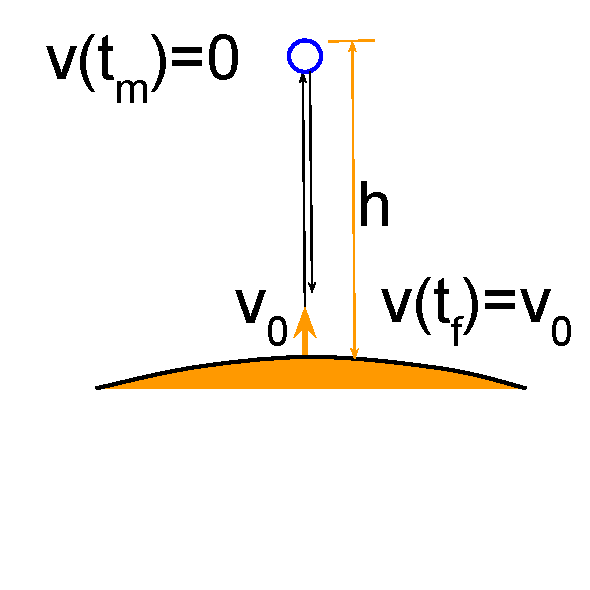
\includegraphics[width=\linewidth]{ParticulaVertical.pdf}
  \caption{Una part\'\i{}cula es lanzada verticalmente hacia arriba con una velocidad inical de $v_{0}$, alcanza una altura m\'axima y vuelve a caer.}
  \label{fig:particula_campo_gravitatorio}
\end{marginfigure}
%%%%%%%%%%%%%%%%

\begin{equation}
\vec{v}(t)=(v_{0}-gt)\hat{z}
\label{eq:particula_vertical_2}
\end{equation}

Cuando la part\'\i{}cula alcanza el punto m\'as alto antes de volver a bajar, la velocidad se hace cero. En ese momento el tiempo marca $t_m=v_0/g$ y la part\'\i{}cula se halla a una altura $h=v_0^2/2g$. Podemos calcular el trabajo realizado considerando separamente el camino de subida y el de bajada
\begin{equation}
W=\int_{0}^{t_f} \vec{F}(t)d\vec{r}=\int_{0}^{t_m} \vec{F}(t)d\vec{r}+\int_{t_m}^{t_f} \vec{F}(t)d\vec{r}
\label{eq:particula_vertical_trabajo}
\end{equation}
Si sustituimos $\vec{F}=-mg\hat{z}$ nos queda
\begin{equation}
W=-\int_{0}^{h} mg dz-\int_{h}^{0} mg dz=-mg(h-0)-mg(0-h)=0
\label{eq:particula_vertical_trabajo_2}
\end{equation}

%%%%%%%%%%


\begin{marginfigure}
  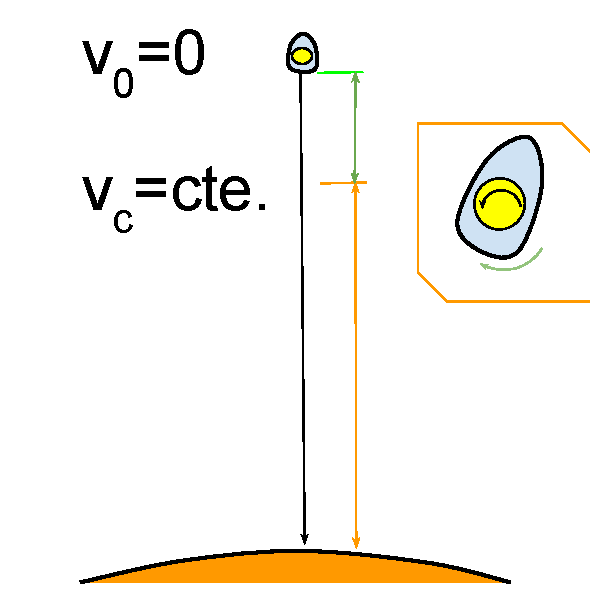
\includegraphics[width=\linewidth]{HuevoSuicida.pdf}
  \caption{Caida libre de un huevo. A partir de una cierta altura el rozamiento del aire compensa la aceleraci\'on de la gravedad y el descenso se produce a velocidad constante.}
  \label{fig:huevo_suicida}
\end{marginfigure}
%%%%%%%%%%%%%%%%

La energ\'\i{}a potencial gravitatoria  entre dos part\'\i{}culas de masas $m$ y $M$ se puede calcular a partir de las ecs. \ref{eq:gravitacion_2} y \ref{eq:energia_potencial}, integrando y asignando el valor cero a la energ\'\i{}a potencial a distancias muy grandes ($r=\infty$)

\begin{equation}
U(\vec{r})=\int_{\infty}^{r}F(r_1)dr_1=GmM\int_{\infty}^{r}\frac{1}{r_1^2}=-G\frac{mM}{r}
\label{eq:energia_potencial_general}
\end{equation}

que ser\'\i{}a equivalente al trabajo necesario para trasladar $m$ desde el punto $r$ hasta una distancia enormemente grande ($\infty$). 

Una pregunta que suele intrigar a los estudiantes que ven por primera vez la ec. \ref{eq:energia_potencial_general} es el significado del signo negativo. Desde el punto de vista del c\'alculo, el signo aparece porque hemos determinado que la energ\'\i{}a potencial gravitatoria valga $0$ cuando $r=\infty$. Pod\'\i{}amos haber tomado otro criterio, por ejemplo, que valiese $0$ en $r=0$ y en ese caso la expresi\'on ser\'\i{}a positiva. En realidad s\'olo las diferencias de energ\'\i{}a entre dos puntos tienen significado, no su valor absoluto.
%%%%%%%%%%


\begin{marginfigure}
  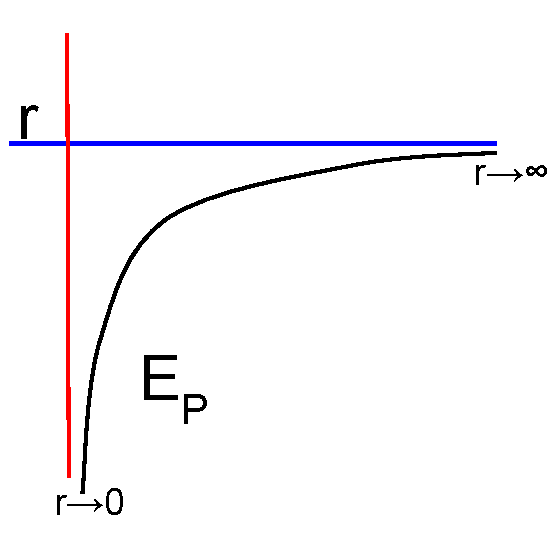
\includegraphics[width=\linewidth]{EnergiaPotencial.pdf}
  \caption{Energ\'\i{}a potencial gravitatoria de una part\'\i{}cula en funci\'on de la distancia. La energ\'\i{}a vale $0$ cuando nos alejamos mucho de la masa que causa el campo gravitatorio. }
  \label{fig:energia_potencial_gravitatoria}
\end{marginfigure}
%%%%%%%%%%%%%%%%

Sin embargo, fijar que la referencia cuando $r=\infty$ o, lo que es equivalente, el signo menos, es importante ya que nos informa de que $m$ est\'a perdiendo energ\'\i{}a potencial conforme se acerca a $r=0$, ciertamente ya que se est\'a acelerando y, por lo tanto, aumentando su energ\'\i{}a cin\'etica.

No todos los campos de fuerzas son conservativos. Imaginemos un \emph{huevo} cayendo en el vac\'\i{}o desde una cierta altura. Al cabo de un cierto tiempo de ca\'\i{}da la resistencia del aire compensa exactamente la aceleraci\'on de la gravedad (no hay fuerza neta sobre el cuerpo), por lo que alcanza una velocidad constante. Por lo tanto no hay trabajo realizado sobre el cuerpo. Como la velocidad no aumenta, tampoco lo hace la energ\'\i{}a cin\'etica. Sin embargo la energ\'\i{}a potencial va disminuyendo conforme el cuerpo se acerca a la Tierra. ?`Acaso no deber\'\i{}a conservarse la energ\'\i{}a mec\'anica de tal modo que $E=U+T=cte$? En este caso la ec. \ref{eq:conservacion_energia_total} no es aplicable porque \emph{no se trata de una masa puntual} sino de un cuerpo extenso que puede tener mecanismos que disipen energ\'\i{}a como la fricci\'on con el aire o la disipaci\'on por rozamiento entre la yema y la clara del huevo. Este tipo de situaciones nos llevan a la necesidad de tener que ampliar nuestro punto de vista.



En 1804 el conde de Rumford observ\'o el  calentamiento que experimentaban los ca\~{n}ones cuando se perforaba el \'anima\cite{Count1804}. Este fen\'omeno no pod\'\i{}a ser debido a la liberaci\'on de ninguna sustancia material sino a la transformaci\'on del movimiento. Posteriormente el cervecero James P. Joule\cite{Joule1850}, un industrial por tradicci\'on familiar y cient\'\i{}fico por afici\'on, llev\'o a cabo un curioso experimento que demostraba la equivalencia entre la energ\'\i{}a mec\'anica y el calor, tal y como se muestra en la fig. \ref{fig:JouleApparatus}. La energ\'\i{}a potencial se puede transformar en energ\'\i{}a cin\'etica y \'esta a su vez en calor, aumentando la temperatura del agua.


El concepto de energ\'\i{}a va m\'as all\'a de la mec\'anica y anunciaba el nacimiento de una nueva disciplina, la \emph{termodin\'amica}.




\section{Intensidad del campo gravitatorio}
Ser\'\i{}a muy c\'omodo aislar esta propiedad que asignamos al espacio que rodea a una masa de la presencia o no de otra masa de prueba. Para ello definimos la \emph{intensidad del campo gravitatorio} producido por la masa $m$ en el punto P como la fuerza por unidad de masa colocada en ese punto

\begin{equation}
\vec{g}=\frac{\vec{F}}{m}=-G\frac{M}{r^2}\hat{r}
\label{eq:intensidad_campo_gravitatorio}
\end{equation}

Luego $g$ tiene sentido opuesto al vector unitario $\hat{r}$, el cual se dirige de la masa que produce el campo al punto donde se calcula el campo. Podemos asociar con cada punto en el espacio alrededor de $M$ un vector $\vec{g}$ que describe el efecto del campo gravitatorio sobre la masa $m$ que coloquemos en el punto. 

%%%%%%%%%%


\begin{marginfigure}
  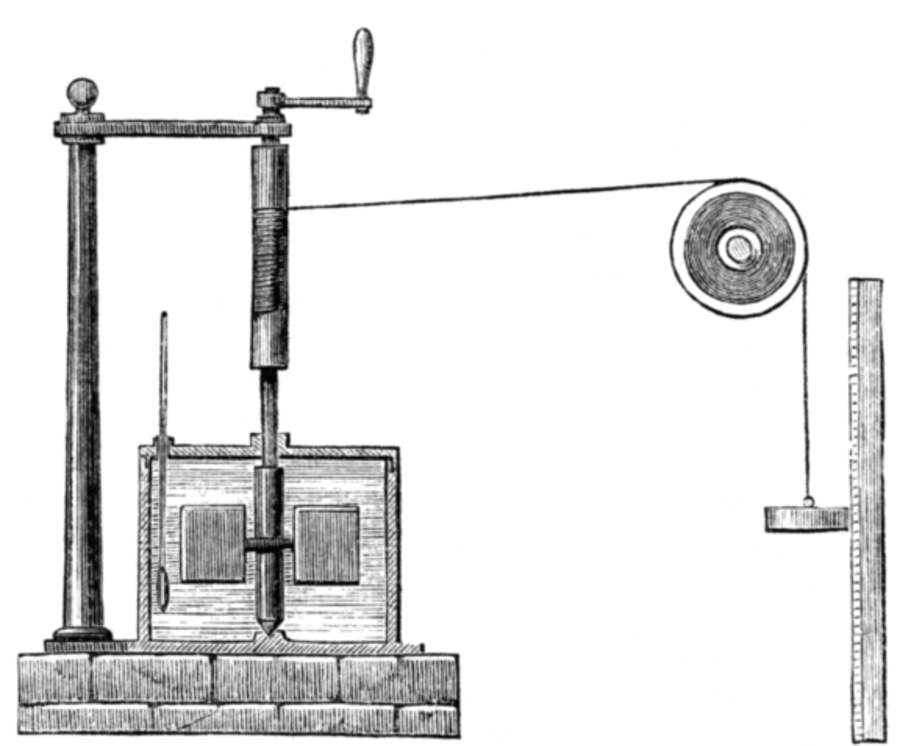
\includegraphics[width=\linewidth]{JouleApparatus.pdf}
  \caption{Aparato de Joule para la medida del equivalente mec\'anico del calor. Joule demostr\'o que el calor necesario para elevar la temperatura de 1 kg de agua de $15\celsius$ a $16\celsius$ equivale a la energ\'\i{}a potencial de 427 kg que se encuentren a la altura de 1 metro sobre el suelo.}
  \label{fig:JouleApparatus}
\end{marginfigure}
%%%%%%%%%%%%%%%%

De la definici\'on vemos que $g$ es equivalente a una aceleraci\'on (se mide en $Nkg^{-1}$ o $ms^{-2}$). Si comparamos las ecuaciones \ref{eq:intensidad_campo_gravitatorio} y \ref{eq:definicion_peso} observamos que la acelaraci\'on de la gravedad puede considerarse como la intensidad del campo gravitacional en la superficie de la Tierra.

\begin{marginfigure}
  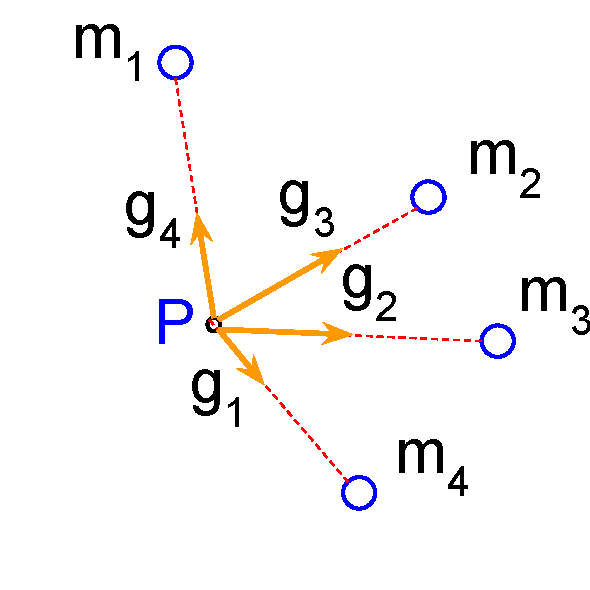
\includegraphics[width=\linewidth]{CampoGravitatorioVariasMasas.pdf}
  \caption{Campo gravitatorio resultante creado por la presencia de varias masas.}
  \label{fig:CampoGravitatorioVariasMasas}
\end{marginfigure}

En el caso de que tuvi\'esemos varias masas  produciendo cada una de ellas su propio campo gravitatorio (fig. \ref{fig:CampoGravitatorioVariasMasas}), la fuerza total ejercida sobre una part\'\i{}cula de masa $m$ situada en el punto P vendr\'\i{}a descrita por 

\begin{equation}
\vec{F}=m\vec{g}_1+m\vec{g}_2+...+m\vec{g}_n=mG\sum_{i=1}^{n}\frac{m_i}{r_i^2}\vec{u}_{ri}
\label{eq:FuerzaCampoGravitatorioVariasMasas}
\end{equation}

Este principio se cumple siempre que tengamos varias masas puntuales y se denomina \emph{principio de superposici\'on}. De forma an\'aloga se puede escribir que el campo creado por estas masas vendr\'\i{}a dado por

\begin{equation}
\vec{g}=\vec{g}_1+\vec{g}_2+...+\vec{g}_n=G\sum_{i=1}^{n}\frac{m_i}{r_i^2}\vec{u}_{ri}=m\frac{vec{F}}{m}
\label{eq:CampoGravitatorioVariasMasas}
\end{equation}

\section{Potencial gravitatorio}
Para un campo de fuerzas conservativo\cite{Golwala2007}, si derivamos la ec. \ref{eq:energia_potencial} con respecto al tiempo podemos escribir de un modo diferente la relaci\'on entre fuerza y energ\'\i{}a potencial
\begin{equation}
\frac{d}{dt}U=-\int_0^{\vec{r}} \frac{d\vec{F}(\vec{r}_1)}{dt} \cdot d\vec{r}_1 -\int_0^{\vec{r}}\vec{F}(\vec{r}_1) \cdot \frac{d}{dt} (d\vec{r}_1)
\label{eq:gradiente_energia_potencial}
\end{equation}
El primer t\'ermino es cero ya que $\vec{F}$ no var\'\i{}a con el tiempo. Por lo tanto 
\begin{equation}
\frac{d}{dt}U= - \vec{F} \cdot \frac{d\vec{r}}{dt}
\label{eq:gradiente_energia_potencial_2}
\end{equation}
El lado izquierdo de la ecuaci\'on \ref{eq:gradiente_energia_potencial_2} podemos reescribirlo como
\begin{equation}
\frac{\partial U}{\partial x}\frac{dx}{dt}+\frac{\partial U}{\partial y}\frac{dy}{dt}+\frac{\partial U}{\partial z}\frac{dz}{dt}= - \vec{F} \cdot \vec{v}
\label{eq:gradiente_energia_potencial_3}
\end{equation}
adoptando una forma similar al producto escalar de dos vectores, uno de ellos ser\'\i{}a $\vec{v}$ y el otro 
\begin{equation}
\vec{\nabla} \equiv \uvec{\i} \frac{\partial}{\partial x}+ \uvec{\j} \frac{\partial}{\partial y}+\uvec{k} \frac{\partial}{\partial z}
\label{eq:definicionGradiente}
\end{equation}
es el \emph{vector gradiente} de modo que
\begin{equation}
- \vec{\nabla} U \cdot \vec{v}=  \vec{F} \cdot \vec{v}
\label{eq:gradiente_energia_potencial_4}
\end{equation} 
Esta expresi\'on deber\'\i{}a ser v\'alida para cualquier valor de $\vec{v}$, de modo que obtenemos la expresi\'on m\'as general 
\begin{equation}
- \vec{\nabla} U =  \vec{F} 
\label{eq:gradiente_energia_potencial_Fuerza}
\end{equation}
que expresa que en un campo de fuerzas conservativo, el gradiente de la energ\'\i{}a potencial es el opuesto de la fuerza que act\'ua sobre la part\'\i{}cula. 

Si definimos el \emph{potencial gravitatorio} como la energ\'\i{}a potencial por unidad de masa colocada en el campo gravitacional
\begin{equation}
V=U/m
\label{eq:definicion_potencial_gravitatorio}
\end{equation}
de las ecs. \ref{eq:intensidad_campo_gravitatorio} y \ref{eq:gradiente_energia_potencial_4} se deduce que
\begin{equation}
- \vec{\nabla} V =  \vec{g} 
\label{eq:gradiente_potecial_intensidad_campo}
\end{equation}
es decir, el campo gravitatorio es el gradiente con signo negativo del potencial gravitatorio. Los puntos con el mismo valor de potencial gravitatorio reciben el nombre de \emph{superficies equipotenciales}. 
El vector gradiente indica la direcci\'on en la que tiene lugar el mayor cambio en $V$. En el caso de los campos gravitatorios originados por part\'\i{}culas puntuales, el  mayor cambio se produce en direcci\'on radial.
Esto implica que tanto $\vec{F}$ como $\vec{g}$  ser\'an perpendiculares a las superficies equipotenciales.

Calculemos la diferencia de potencial entre los puntos A y B de la figura \ref{fig:DiferenciaPotencialAB}

\begin{equation}
V_A-V_B=\frac{U(\vec{r}_A)-U(\vec{r}_B)}{m}=\int_A^B\frac{\vec{F}}{m} d\vec{r}=
\label{eq:diferenciaPotencialAB}
\end{equation}
Si sustituimos $\vec{F}$ de acuerdo con la ec. \ref{eq:gravitacion_2}
\begin{equation}
V_A-V_B=-GM \int_A^B \frac{1}{r^2}dr
\label{eq:diferenciaPotencialAB_2}
\end{equation}
e integramos
\begin{equation}
V_A-V_B=-GM\left[ -\frac{1}{r}\right]_A^B=\left(-G\frac{M}{r_A}\right)-\left(-G\frac{M}{r_B}\right)
\label{eq:diferenciaPotencialAB_22}
\end{equation}
Podemos elegir como $0$ el valor del potencial a distancia infinita de la masa $M(r\rightarrow \infty)$, de ese modo
\begin{equation}
V=-G\frac{M}{r}
\label{eq:PotencialAB}
\end{equation}
De la ec. (\ref{eq:PotencialAB}) es posible concluir que el potencial gravitatorio en un punto del espacio es el trabajo que realiza el campo gravitatorio para trasladar la unidad de masa desde dicho punto hasta el infinito.


Ambos puntos, $A$ y $B$, est\'an situados a diferentes distancias de la masa $M$ que origina el campo gravitatorio, es decir, estar\'\i{}an en diferentes superficies equipotenciales. Como hemos explicado previamente (fig. \ref{fig:campo_gravitatorio}), las superficies equipotenciales son esferas conc\'entricas cuyos centros est\'an situados en el punto donde se halla la part\'\i{}cula puntual $M$. 

A partir de la ecuaci\'on \ref{eq:diferenciaPotencialAB_22} resulta evidente que la diferencia de potencial entre los puntos A y C tiene que ser cero.


\begin{marginfigure}
  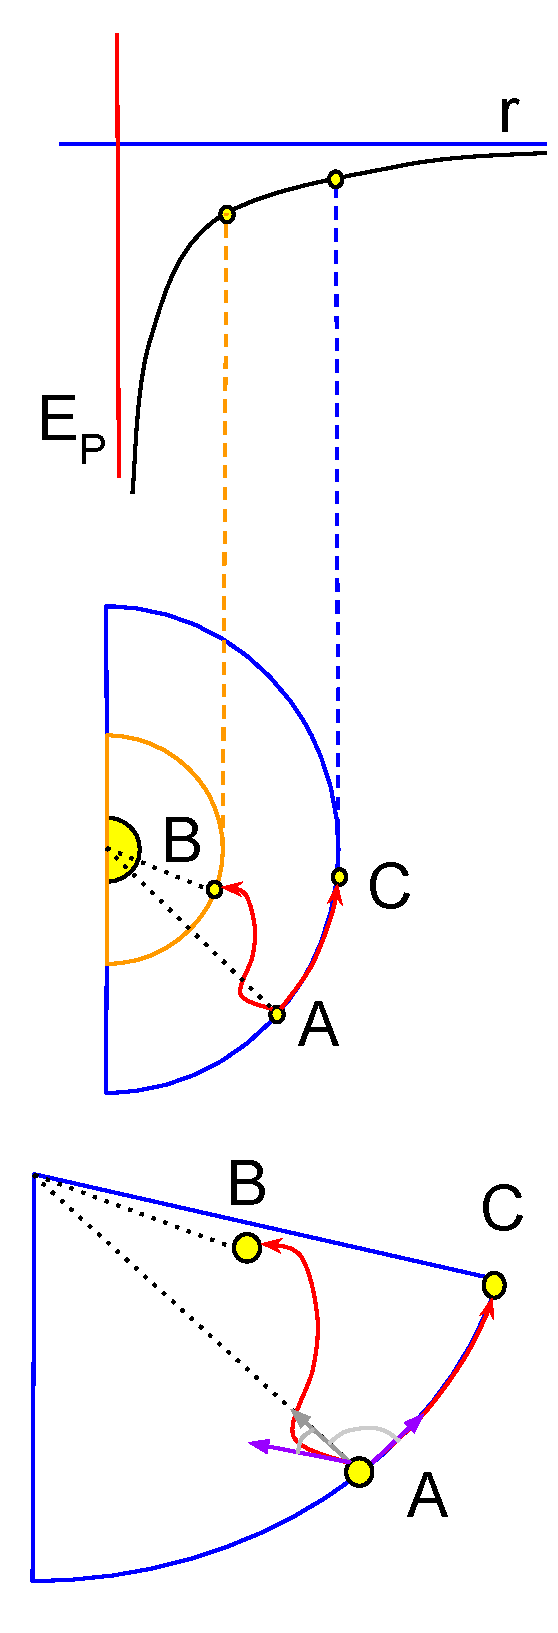
\includegraphics[width=\linewidth]{DiferenciaPotencialAB.pdf}
  \caption{Diferencia de potencial entre 2 puntos situados a diferentes distancias de la masa puntual $M$.}
  \label{fig:DiferenciaPotencialAB}
\end{marginfigure}
Debe tenerse en cuenta que el potencial, a diferencia del campo, es una magnitud escalar. Si en lugar de una part\'\i{}cula tenemos varias (fig. \ref{fig:CampoGravitatorioVariasMasas}), el potencial se calcular\'\i{}a sumando escalarmente el potencial creado en ese punto por cada part\'\i{}cula, de acuerdo con la ecuaci\'on \ref{eq:energia_potencial_general}
\begin{equation}
V=V_1+V_2+...+V_n=-G\sum_{i=1}^{n}\frac{m_i}{r_i}
\label{eq:potencial_varias_particulas}
\end{equation}

\section{El campo gravitatorio debido a masas no puntuales. Cuerpos esf\'ericos}

Hasta ahora hemos utilizado con alegr\'\i{}a la aproximaci\'on de que el tama\~no de los planetas era muy peque\~no en comparaci\'on con las distancias que los separan (masas puntuales). Pero, ?`realmente es siempre as\'\i{}??`C\'omo afecta a las expresiones deducidas el hecho de que los planetas tengan un tama\~no finito? Newton mismo estuvo muy preocupado por este hecho y demor\'o la publicaci\'on de su ley de gravitaci\'on durante unos 20 a \~nos hasta que encontr\'o la explicaci\'on correcta 
%(citar realci\'on con el desarrollo del c\'alculo infinitesimal). 

Calcular el campo creado por una esfera maciza no es un problema f\'acil (!`al propio Newton le llev\'o d\'ecadas dar con la soluci\'on m\'as simple!). Para resolverlo, comencemos por algo sencillo. Esta es una t\'ecnica muy \'util; si no somos capaces de hallar la soluci\'on de un problema complejo, intent\'emoslo con uno m\'as simple (es el viejo truco, si no te hace caso la m\'as guapa de la fiesta, o el m\'as guapo, lo intentamos con su amiga ). En este caso la simplificaci\'on consiste en imaginar el campo creado por una capa esf\'erica\cite{AlonsoFin1986}. Podemos imaginarlo como la c\'ascara de una naranja. Posteriormente supondremos que una esfera maciza puede dividirse imaginariamente en un conjunto de c\'ascaras esf\'ericas conc\'entricas y sumar.

%%%%%%%%%%%%%%%%%%
\begin{figure*}[h]
  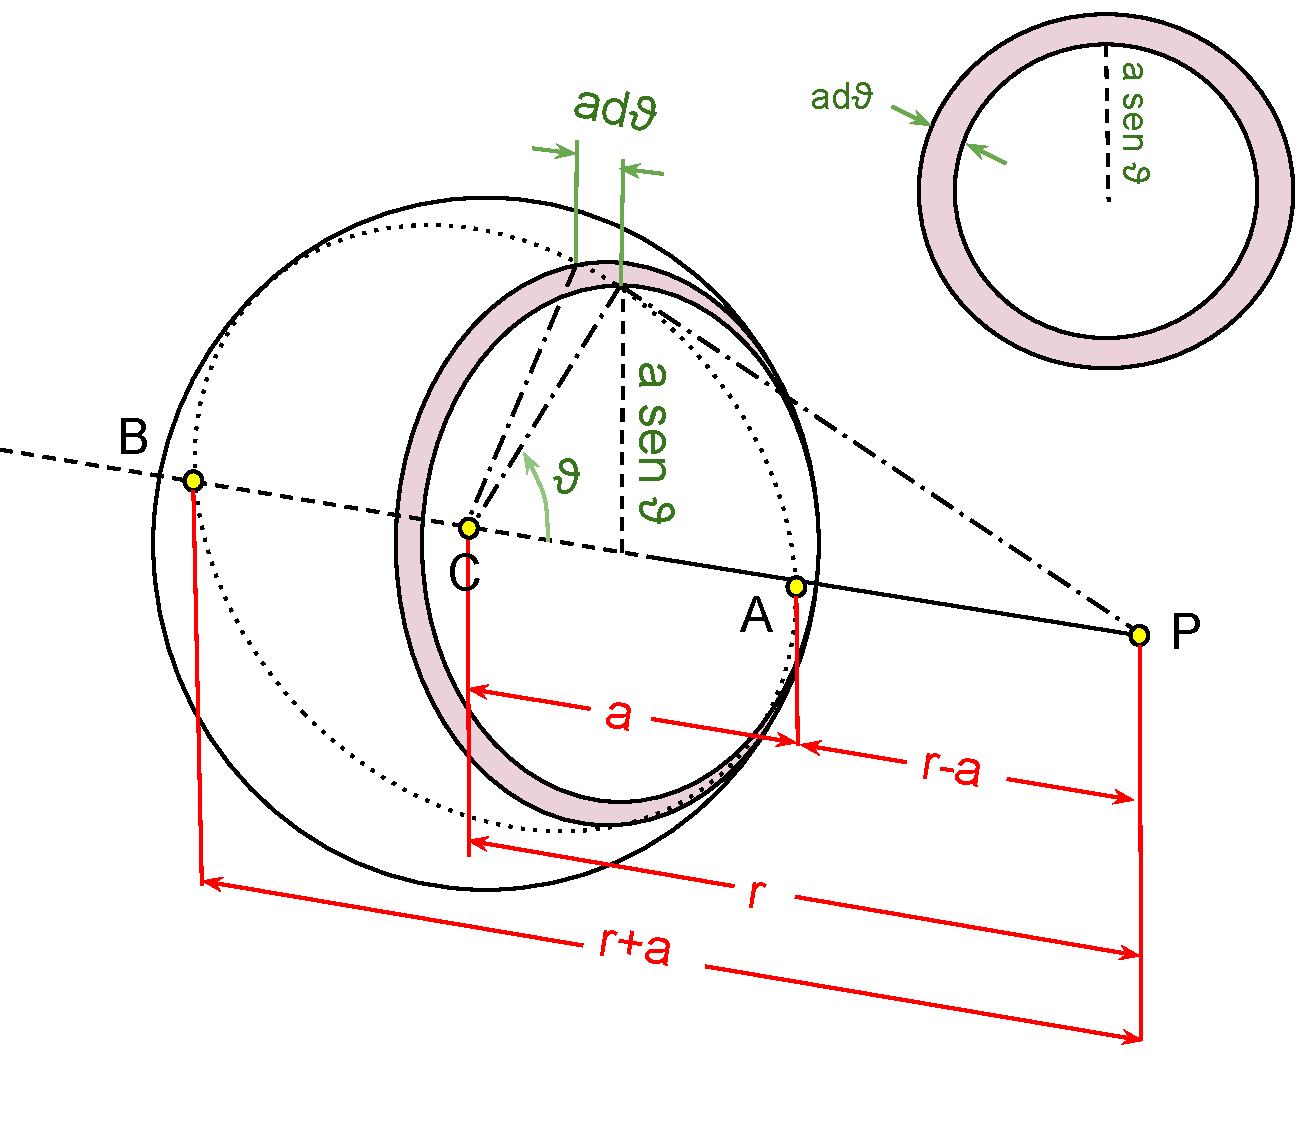
\includegraphics[width=\linewidth]{EsferaGravedad.pdf}
  \caption{C\'alculo del campo gravitatorio en un punto externo a una masa uniformemente distribuida en una capa esf\'erica.}
  \label{fig:EsferaGravedad}
\end{figure*}
%%%%%%%%%%%%%%%

De acuerdo con el dibujo de la Fig. \ref{fig:EsferaGravedad}, la esfera de radio $a$ est\'a situada a una distancia $P$ de un punto arbitrario. $C$ es el centro de la esfera y los puntos $A$ y $B$ son los puntos en los que cortar\'\i{}a a la  esfera la recta $CP$. Si con una cuchilla afilada cort\'asemos la c\'ascara por dos planos paralelos entre s\'\i{}  y perpendiculares a $CP$ obtendr\'\i{} amos una zona circular estrecha. El \'area de la zona vendr\'\i{}a dada por
\begin{equation}
A= (2 \pi a \sin \theta)(a d\theta)
\label{eq:area_zona_circular}
\end{equation}
Si $m$ es la masa total de superficie de la esfera (supongamos que es homog\'enea), la masa por unidad de \'area ser\'\i{}a
\begin{equation}
\frac{m}{4 \pi a^2}
\label{eq:masa_area}
\end{equation}
y la masa de la zona circular 
\begin{equation}
\frac{m}{4 \pi a^2}(2 \pi a^2 \sin \theta d \theta)=\frac{1}{2}m \sin \theta d \theta
\label{eq:masa_area_circular}
\end{equation}
Todos los puntos situados en la zona se encuentran a una distancia $R$ del punto $P$. Si utilizamos la ecuaci\'on \ref{eq:PotencialAB}, podemos escribir el potencial gravitatorio creado por la zona circular en $P$

\begin{equation}
dV=-G\frac{m \sin \theta d \theta}{2R}=-G\frac{m}{2R}\sin \theta d\theta
\label{eq:potencial_masa_area_circular}
\end{equation}
De la figura \ref{fig:EsferaGravedad}, utilizando la ley de los cosenos\footnote{$a²=b²+c²-2bc \cos A$}.
\begin{equation}
R^2= a^2+r^2-2ar \cos \theta
\label{eq:ley_cosenos_aplicada_esfera}
\end{equation}
Diferenciando la ec. \ref{eq:ley_cosenos_aplicada_esfera} y teniendo en cuenta que $a$ y $r$ son constantes nos queda
\begin{equation}
2RdR=2 a r \sin \theta d \theta
\label{eq:der_ley_cosenos_aplicada_esfera}
\end{equation}
Si despejamos $\sin \theta d \theta$ y sustituimos en la ecuaci\'on \ref{eq:potencial_masa_area_circular} se obtiene
\begin{equation}
dV=-G\frac{m}{2ar}dR
\label{eq:potencial_masa_area_circular_2}
\end{equation}

Imaginemos la superficie de la esfera como la suma de un mont\'on de estas zonas circulares. Bastar\'\i{}a con sumar la contribuci\'on de cada una de ellas al c\'alculo de potencial, lo que matem\'aticamente equivale a hacer la integral (tal y como se muestra en la animaci\'on\cite{Newton2006})
\begin{equation}
V=-G\frac{m}{2ar}\int _{r-a}^{r+a}dR=-G\frac{m}{2ar}(2a)=-G\frac{m}{r}
\label{eq:potencial_masa_area_circular_3}
\end{equation}
donde suponemos que $r>a$, es decir, que $P$ est\'a fuera de la esfera.  Si $P$ estuviera dentro de la esfera, los l\'\i{}mites de integraci\'on cambiar\'\i{}an
\begin{equation}
V=-G\frac{m}{2ar}\int _{a-r}^{a+r}dR=-G\frac{m}{2ar}(2r)=-G\frac{m}{a}
\label{eq:potencial_masa_area_circular_4}
\end{equation}
que es constante, independiente de la posici\'on de $P$. Podemos pasar a las expresiones equivalentes para el campo gravitatorio $\vec{g}$ mediante la ec. \ref{eq:gradiente_potecial_intensidad_campo}, en la que utilizamos la idea de gradiente
\begin{equation}
\vec{g}=-G\frac{m}{r^2}\hat{r}
\label{eq:campo_masa_area_circular_1}
\end{equation}
que nos dar\'\i{}a el campo cuado $r>a$ y
\begin{equation}
\vec{g}=0
\label{eq:campo_masa_area_circular_2}
\end{equation}
cuando $r<0$. Si se examina con detalle la forma de la c\'ascara esf\'erica, cada sector diferencial de la misma contribuye creando un campo que se compensa exactamente por el sector sim\'etrico con respecto al centro.  En res\'umen, \emph{el campo gravitatorio y el potencial creado por una capa esf\'erica en un punto exterior a la misma es id\'entica a la que crear\'\i{}a una part\'\i{}cula de la misma masa situada en el centro de la esfera. En cuanto al interior, el campo es cero y el potencial constante.} En las figura \ref{} se puede ver la variaci\'on del potencial y el campo con la distancia al centro de la esfera.

El paso final consiste en imaginar que una esfera maciza es la superposici\'on de un n\'umero suficientemente grande de estas c\'ascaras esf\'ericas situadas de forma conc\'entrica, como las capas de una cebolla. Cada capa produce un campo dado por las ecuaciones \ref{eq:campo_masa_area_circular_1} y \ref{eq:campo_masa_area_circular_2}. Como la distancia $r$ es la misma para todas las capas conc\'entricas, las ecuaciones siguen siendo v\'alidas para esferas macizas. Por consiguiente, \emph{una esfera s\'olida origina en puntos externos a ella un campo gravitatorio y un potencial id\'enticos a los que provocar\'\i{} a una part\'\i{} cula con la misma masa situada en el centro de la esfera}.

Existe otro modo justificar este resultado, utilizando para ello el concepto de flujo gravitatorio. Se define el \emph{flujo gravitatorio} a trav\'es de una superficie como
\begin{equation}
\phi =\int_S \vec{g} \cdot  d\vec{S}
\label{eq:flujo_gravitatorio}
\end{equation}

Si imaginamos el campo como un conjunto de l\'\i{}neas que parten de la masa (puntual o no), y la rodeamos de una esfera imaginaria, el n\'umero total de l\'\i{}neas que cortan la superficie es siempre el mismo, depende sólo de la masa y es independiente del radio de la esfera. A este resultado general se le conoce por el nombre de \emph{Teorema de Gauss}\footnote{Tambi\'en conocido por teorema de la divergencia}. 

\begin{equation}
\phi =\int_S \vec{g} \cdot  d\vec{S}=-4 \pi G M
\label{eq:teorema_gauss_gravitatoria_1}
\end{equation}

Aplicando el resultado \ref{eq:teorema_gauss_gravitatoria} a una superficie gaussiana $S$ en forma de esfera conc\'entrica con la distribuci\'on de masa y que contenga al punto $P$ en el que calculamos el campo (v\'ease fig. \ref{})
\begin{equation}
\phi =\int_S \vec{g} \cdot  d\vec{S}=-\int_S g dS=-g \int_S  dS= -g 4 \pi r^2
\label{eq:teorema_gauss_gravitatoria_2}
\end{equation}
ya que $\vec{g}$ es perpendicular a la superficie $S$ en todos sus putnos y su m\'odulo es constante sobre $S$. Utilizando el teorema de la divergencia de gauss (ec. \ref{eq:teorema_gauss_gravitatoria_1}) obtenemos

\begin{equation}
 -g 4 \pi r^2=-4 \pi G M
\label{eq:teorema_gauss_gravitatoria_3}
\end{equation}
de donde podemos despejar $g$

\begin{equation}
g=G\frac{M}{r^2}
\label{eq:modulo_campo_esfera}
\end{equation}
y de esta expresi\'on podr\'\i{} amos calcular el potencial.

%%%%%%%%%%%%%%%%%%%%%%%%%%%%%%%%%%%%%%%%%%%%%%%%%%%

%%%%%%%%%%%%%%%%%%%%%%%%%%%%%%%%%%%%%%%%%%%%%%%%%%%%

%%%%%%%%%%%%%%%%%%%%%%%%%%%%%%%%%%%%%%%%%%%%%%%%%%%
%%%%%%%%%%%%%%%%%%%%%%%%%%%%%%%%%%%%%%%%%%%%%%%%%%%

\section{Relaci\'on entre energ\'\i{}a y movimiento orbital}

La energ\'\i{}a total de un sistema de dos part\'\i{}culas sometidas \'unicamente a su interacci\'on gravitatoria ser\'a la suma de sus energ\'\i{}as cin\'etica y gravitatoria

\begin{equation}
E=\frac{1}{2}mv^2+\frac{1}{2}Mv^2-G\frac{mM}{r}
\label{eq:energia_total_gravitatoria_2p}
\end{equation}

Si suponemos que una de ellas es mucho m\'as grande que la otra ($M\gg m$), y fijamos el origen del sistema de coordenadas en la part\'\i{}cula mayor, \'esta se hallar\'\i{}a en reposo y la energ\'\i{}a total se escribir\'\i{}a
\begin{equation}
E=\frac{1}{2}mv^2-G\frac{mM}{r}
\label{eq:eenergia_total_gravitatoria_Masa_grande}
\end{equation}
Si la part\'\i{}cula se mueve en una \'orbita circular, la fuerza que act\'ua sobre ella viene dada por la ecuaci\'on \ref{eq:fuerza_centripeta}
\begin{equation}
\frac{mv^2}{r}=-G\frac{mM}{r^2}
\label{eq:fuerza_centripeta_gravedad}
\end{equation}
Sustituyendo en la ecuaci\'on \ref{eq:eenergia_total_gravitatoria_Masa_grande}
\begin{equation}
E=\frac{1}{2}mv^2-G\frac{mM}{r}=\frac{1}{2}G\frac{mM}{r}-G\frac{mM}{r}=-\frac{1}{2}G\frac{mM}{r}<0
\label{eq:eenergia_total_orbitacircular}
\end{equation}
concluimos que la energ\'\i{}a total es negativa. Este resultado no es solamente v\'alido para las \'orbitas circulares; todas las \'orbitas cerradas tiene una energ\'\i{}a total negativa cuando fijamos el valor de la energ\'\i{}a potencial a cero para distancias infinitas (fig. \ref{fig:EnergiaTrayectoria}). Una \'orbita cerrada significa que la energ\'\i{}a cin\'etica de la part\'\i{}cula no es suficientemente grande en ning\'un punto de la \'orbita como para llevar la part\'\i{}cula al infinito. En ese punto el segundo t\'ermino de la ecuaci\'on \ref{eq:eenergia_total_gravitatoria_Masa_grande} vale $0$. 
Si la energ\'\i{}a total vale $0$ nos encontramos ante el caso l\'\i{}mite que separa trayectorias cerradas de aquellas en las que el cuerpo logra escapar.
%%%%%%%%%%%%%%%
\begin{figure*}[h]
  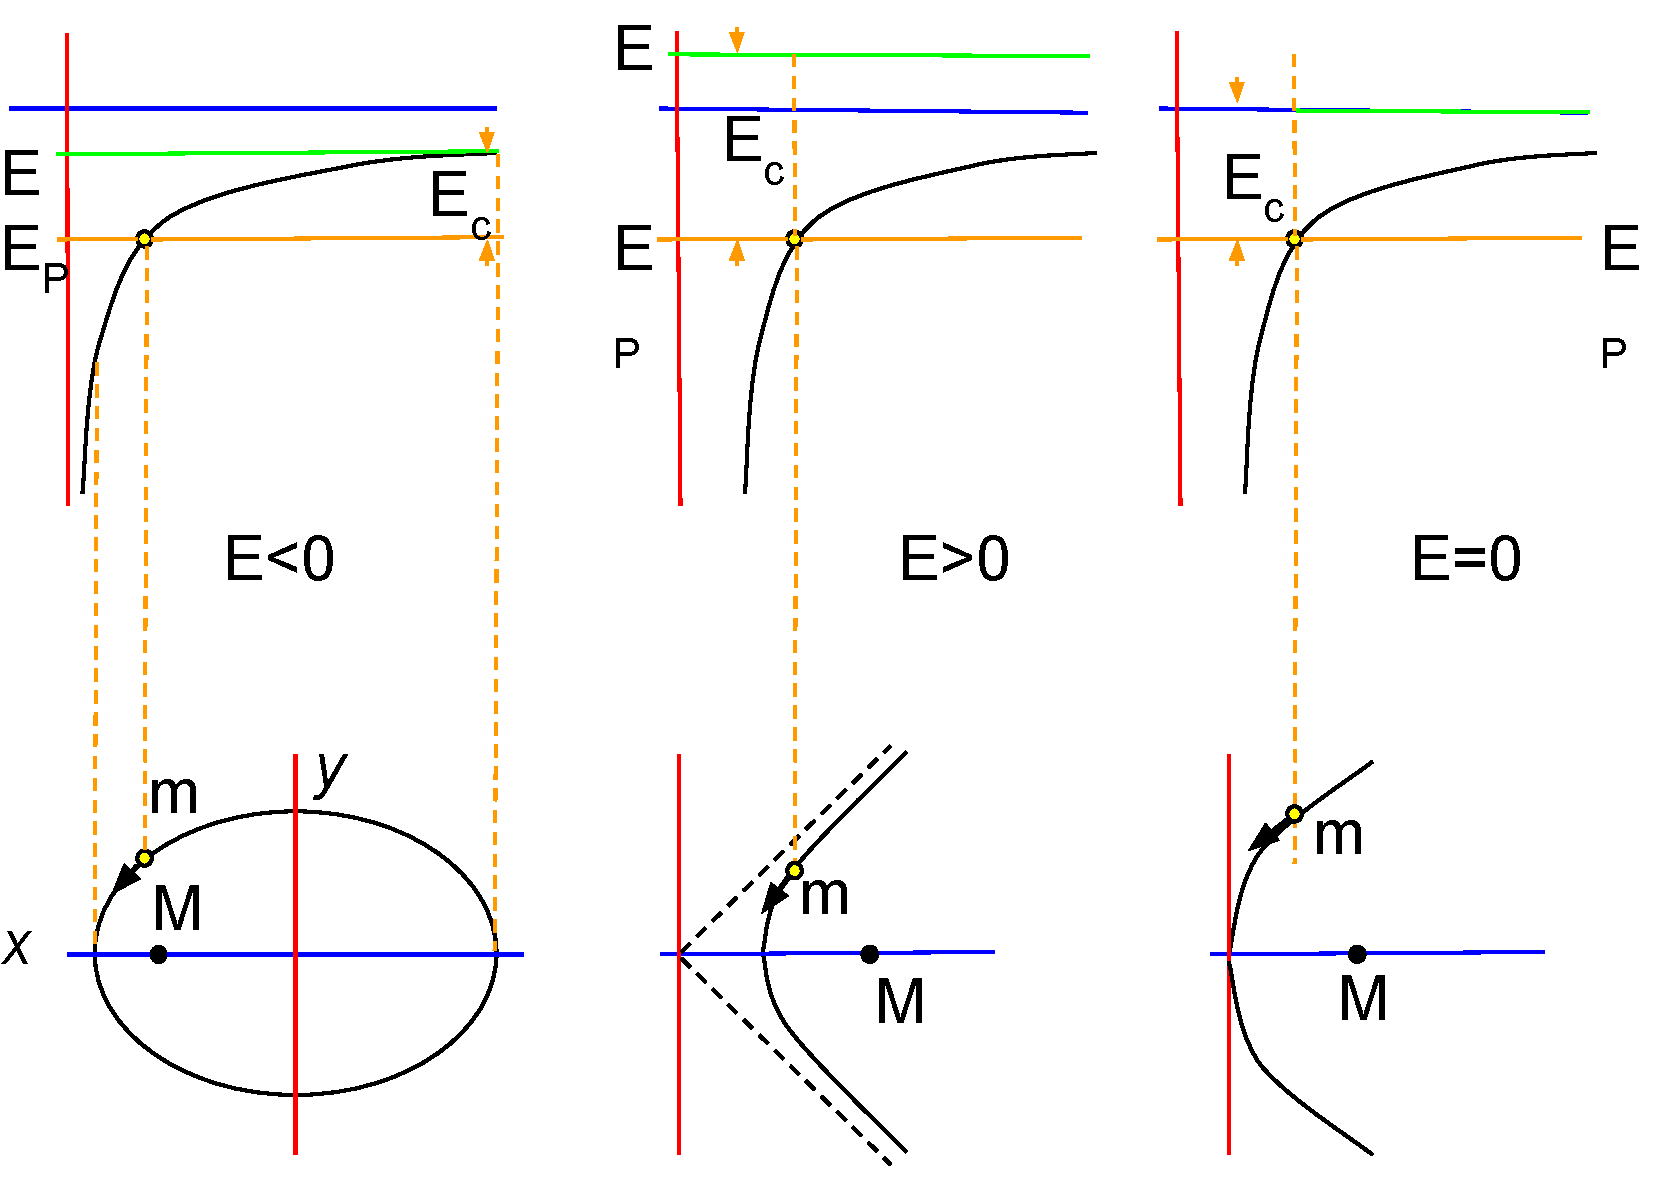
\includegraphics[width=\linewidth]{EnergiaTrayectoria.pdf}
  \caption{Relaci\'on entre la energ\'\i{}a total y la trayectoria en el movimiento de una masa en torno a otra.}
  \label{fig:EnergiaTrayectoria}
\end{figure*}
%%%%%%%%%%%%%%%


\section{Caos determinista}


